\documentclass{article}
\usepackage{amsmath}
\usepackage[margin=0.5in]{geometry}
\usepackage{breakcites}
\usepackage{natbib}
\usepackage{mathtools}
\usepackage{mathrsfs}
\usepackage{graphicx}
\usepackage{caption}
\usepackage[bottom]{footmisc}
\usepackage[export]{adjustbox}
\usepackage{todonotes}
\usepackage{footnote}
\usepackage{threeparttable}

\usepackage{newfloat}
\DeclareFloatingEnvironment[placement={!ht},name=List]{ordlist}

\usepackage{xr}
\externaldocument[S-]{supplement}

\DeclarePairedDelimiter\ceil{\lceil}{\rceil}
\DeclarePairedDelimiter\floor{\lfloor}{\rfloor}
\DeclareMathAlphabet\mathbfcal{OMS}{cmsy}{b}{n}
\DeclareMathOperator*{\argmin}{arg\,min}

\begin{document}


\newcommand{\monosaccharide}[1]{{\bf #1}}
\newcommand{\nglycan}[0]{\textit{N}-glycan }
\newcommand{\nglycans}[0]{\textit{N}-glycans }

\newcommand{\msn}[0]{$MS^n$}
\newcommand{\ms}[1]{$MS^#1$}

% Sample Name Shortcuts
\newcommand{\agp}[0]{\textit{20150930-06-AGP} }
\newcommand{\phil}[0]{\textit{20141031-07-Phil-82} }
\newcommand{\philbs}[0]{\textit{20141101-04-Phil-BS} }
\newcommand{\igg}[0]{\textit{20151002-02-IGG} }
\newcommand{\dpphil}[0]{\textit{20141128-11-Phil-82} }
\newcommand{\dpagp}[0]{\textit{AGP-DR-Perm-glycans-1} }
\newcommand{\rpagp}[0]{\textit{AGP-permethylated-2ul-inj-55-SLens} }
\newcommand{\rphumanserum}[0]{\textit{Perm-BS-070111-04-Human-Serum} }


\title{Application of Network Smoothing to Glycan LC-MS Profiling}
\author{Joshua Klein}
\begin{abstract}
    \textbf{Motivation:} Glycosylation is one of the most heterogenous
    and complex post-translational modifications, but.\\
    \textbf{Results:} These are the resutls for this article.\\
\end{abstract}

\maketitle

\section{Introduction}
Glycosylation is one of the most pervasive forms of post-translational
modification.


\section{Methods}

\subsection{Glycan Hypothesis Generation}
        In eukaryotes, \nglycans start with a common, conserved core of \textbf{HexNAc2 Hex3},
    building up to \textbf{HexNAc2 Hex9} (\cite{Stanley2009}). This structure is refined by
    sequentially removing monosaccharides and replacing them with more complex structures
    through a series of glycosidase and glycosyltransferase reactions, the enumeration of
    which as shown in \cite{Akune2016} yields over a million of possible \nglycan topologies
    and epitopes. These topologies define the geometry of the glycan, affecting the glycan's
    binding affinities and how the glycan may influence protein folding and accessibility,
    the glycan's functional aspects. The medium through which we observe \nglycan does not
    capture the full tree or graph structure of an \nglycan, so we reduce the topology to
    a count of each type of residue.

        Starting with the core motif, we generate all combinations of monosaccharides ranging
    between the limits in Table \ref{tab:glycan_composition_rules}. We created a copy of
    this database for native, reduced and permethylated, and deuteroreduced and permethylated.
    Let $n = 1240$ be the number of glycan compositions $\mathbf{g}$ in the database.

    \renewcommand{\arraystretch}{1.5}
    \begin{table}
        \centering
        \savenotes
        \caption{Glycan Composition Rule Table}\label{tab:glycan_composition_rules}
        \begin{tabular}{c | c | c | c}
            Monosaccharide & Lower Limit & Upper Limit & Constraints\\
            \hline
            \monosaccharide{HexNAc} & 2 & 9 &\\
            \monosaccharide{Hex} & 3 & 10 & \\
            \monosaccharide{Fuc} & 0 & 4 & $\monosaccharide{HexNAc} > \monosaccharide{Fuc}$\\
            \monosaccharide{NeuAc} & 0 & 5 & $(\monosaccharide{HexNAc} - 1) > \monosaccharide{NeuAc}$\\
        \end{tabular}
        \spewnotes
    \end{table}
    \renewcommand{\arraystretch}{1.0}

\subsection{LC-MS Data Preprocessing}
    We analyzed samples from several sources, including both QTOF and Orbitrap
    instruments as shown in Table \ref{tab:sample_overview}. For details on sample preparation
    and data acquisition, please see the source citations. We converted all
    datasets to mzML format (\cite{Martens2011}) using Proteowizard
    (\cite{Kessner2008}) without any data transforming filters. We applied a background reduction
    method based upon (\cite{Kaur2006}), using a window length of 2 m/z. Next, we picked peaks using
    a simple Gaussian model and iteratively charge state deconvoluted and deisotoped using an
    averagine (\cite{Senko1995}) formula appropriate to the molecule under study. For native
    glycans, the formula was \textbf{H 1.690 C 1.0 O 0.738 N 0.071}, for permethylated glycans,
    the formula was \textbf{H 1.819 C 1.0 O 0.431 N 0.042}. We used an iterative approach which combines
    aspects of the dependence graph method (\cite{Liu2010}) and with subtraction. All samples
    were processed using a minimum isotopic fit score of 20 with an isotopic strictness penalty
    of 2.

    \begin{table}
        \caption{Samples Used}\label{tab:sample_overview}
        \small
        \centering
        \begin{threeparttable}
        \begin{tabular}{p{4.1cm} | c | p{3cm} | p{3cm} | c}
            \toprule
            Sample Name & Instrument & Derivatization & Adduction & Source\\
            \midrule
            20150930-06-AGP & QTOF & Native & Formate (1) & \cite{Khatri2016a}\\
            20141031-07-Phil-82 & QTOF & Native & Formate (3) & \cite{Khatri2016a}\\
            20141103-02-Phil-BS & QTOF & Native & Formate (3) & \cite{Khatri2016a}\\
            20151002-02-IGG & QTOF & Native & Formate (2) & \cite{Khatri2016b}\\
            20141128-11-Phil-82\tnote{1} & QTOF &
                Deutero-reduced and Permethylated & Ammonium (3) & \cite{Khatri2016a}\\
            AGP-DR-Perm-glycans-1\tnote{1} & Orbitrap &
                Deutero-reduced and Permethylated & Ammonium (3) & \cite{Khatri2016a}\\
            AGP-permethylated-2ul-inj-55-SLens\tnote{1} & Orbitrap &
                Reduced and Permethylated & Ammonium (3) & \cite{Khatri2016a}\\
            Perm-BS-070111-04-Serum\tnote{1} & Orbitrap &
                Reduced and Permethylated & Ammonium (3) & \cite{Yu2013,Hu2012}\\
        \end{tabular}
        \begin{tablenotes}
            \item[1] Included $MS^n$ Scans
        \end{tablenotes}
        \end{threeparttable}
    \end{table}


\subsection{Chromatogram Aggregation}
        We cluster peaks whose neutral masses are within 15 parts-per-million error
    (PPM) of each other. When there are multiple candidate clusters for a single peak,
    we use the cluster with the lowest mass error. After all peaks are clustered,
    we sort each cluster by time, creating a list of aggregated chromatograms. To account
    for small mass differences, we find all chromatograms which are within 10 PPM of each
    other and which overlap in time and merge them.

\subsection{Glycan Composition Matching}
        For each chromatogram, we queried the target glycan database for compositions
    whose masses were within $\delta_{mass} = 10$ PPM for QTOF data, $5$ PPM
    for FTMS data. We merged all features matching the same composition. Then, for
    each adduct combination, we searched the target glycan database for compositions
    whose neutral mass were within $\delta_{mass}$ of the observed neutral mass - adduct
    combination mass, followed by another round of merging chromatogramss with the same
    assigned composition. We reduced the data by splitting each feature where the time
    between sequential observation was greater than $\delta_{rt} = 0.25$ minutes and
    removed features with fewer than $k = 5$ data points. For cases where $MS^n$ scans were
    present, these scans were mapped onto their precursor $MS^1$ features, and evaluated for
    glycan-like product ions, retaining only those which satisfied the signature ion
    criterion described in section S\ref{S-sec:signature_ion_criterion}. We term the
    remaining assigned and unassigned chromatograms \textit{candidate features}.


\subsection{Feature Evaluation}
        For each candidate feature, we computed several metrics to estimate
    how distinguishable the observed signal was from random noise. The
    features are mentioned in List~\ref{list:scoring_features}, but for more
    information see Section~S\ref{S-sec:feature_evaluation}.
    \begin{ordlist}
    \begin{enumerate}
        \itemsep0em
        \caption{Chromatographic Feature Metrics\label{list:scoring_features}}
        \item Goodness-of-fit of chromatographic peak shape to a model function
              (\cite{Yu2010,Kronewitter2014}).
        \item Goodness-of-fit of isotopic pattern to glycan composition weighted
              by peak abundance (\cite{Maxwell2012}).
        \item Observed charge states with respect to glycan composition and mass.
        \item Time gap between $MS^1$ observations detecting measuring missing peaks
              and interference.
        \item Adduction states with respect to glycan composition and mass.
    \end{enumerate}
    \end{ordlist}

        These metrics are bounded in $[0, 1)$. Any observation for which any metric
    was observed below $0.15$ was discarded as having insufficient evidence for
    consideration. The \textit{observed score} $s$ for each candidate feature is
    the sum of the logit-transformation of these metrics. This produces a single
    value bounded in $[0, \infty)$, whose distribution we assume is asymptotically
    normal. $s < 8$ reflects a low confidence match, with confidence increasing
    as $s$ does. As these metrics are tied to reliable detection of the the glycan
    by the mass spectrometer, they are dependent upon glycan abundance and sample
    quality and the resolution of the mass spectrometer used.


\subsection{Glycan Composition Network Smoothing}
        Evidence for individual glycan compostions can often be enough to claim
    that composition had been detected. Lower abundance may score poorly in one
    or more features, leading to the glycan composition being discarded. Other
    methods have demonstrated it is advantageous to use relationships between
    glycans based on biosynthetic or structural rules to adjust the score of a
    single glycan assignment (\cite{Goldberg2009, Kronewitter2014}). This idea
    has been explored more generically under the name "Manifold Regularization"
    (\cite{Belkin2006}) and specifically "Laplacian Regularization" when the
    Laplacian matrix of a graph is used to influence the parameter scaling. We
    apply this idea to weighted networks of related glycans with arbitrarily
    defined and overlapping sub-populations.

        \subsubsection{Glycan Composition Graph}
        For each database of theoretical glycan compositions we create, we
        define each composition to be a coordinate vector in a $\mathcal{Z}^{+c}$
        space where $c$ is the number of components in any glycan composition,
        and represented by a node in an undirected glycan composition
        graph $\mathcal{G}$. Under this interpretation, we can compute the
        $L_1$-distance between two glycan compositions. For any two glycan
        compositions $g_u, g_v$, if $L_1(g_u, g_v) = 1$ we add an edge
        connecting $g_u$ and $g_v$ to $\mathcal{G}$ with weight $w = 1$.


        \subsubsection{Neighborhood Definition}
        Our definition of distance connects glycan compositions which differ
        by a single monosaccharide, but we can assert how larger collections of
        glycan compositions are related. To this end, we extend the definition of
        neighborhoods for \nglycans using intervals over monosaccharide counts
        shown in Table~\ref{tab:neighborhood_definitions}. These neighborhoods are
        arranged to span particular epitopes or biosynthetically related
        subtypes of \nglycans, such as sialylation state or branching
        pattern.

        \begin{table}[tb]
            \centering
            \small
            \begin{tabular}[h]{l p{8cm}}
                \toprule
                Name & Bounds \\
                \midrule
                High Mannose & $\monosaccharide{HexNAc} = 2 \land
                                \monosaccharide{Hex} \in [3, 10]
                                \land \monosaccharide{NeuAc} = 0$\\
                Hybrid & $\monosaccharide{HexNAc} \in [2, 4] \land
                          \monosaccharide{Hex} \in [2, 6]
                          \land \monosaccharide{NeuAc} \in [0, 2]$\\
                Bi-Antennary & $\monosaccharide{HexNAc} \in [3, 5]
                                \land \monosaccharide{Hex} \in [3, 6]
                                \land \monosaccharide{NeuAc} \in [1, 3]$\\
                Asialo-Bi-Antennary & $\monosaccharide{HexNAc} \in [3, 5]
                                \land \monosaccharide{Hex} \in [3, 6]
                                \land \monosaccharide{NeuAc} \in [0, 1]$\\
                Tri-Antennary & $
                    \monosaccharide{HexNAc} \in [4, 6]
                    \land \monosaccharide{Hex} \in [4, 7]
                    \land \monosaccharide{NeuAc} \in [1, 4]
                $\\
                Asialo-Tri-Antennary & $
                    \monosaccharide{HexNAc} \in [4, 6]
                    \land \monosaccharide{Hex} \in [4, 7]
                    \land \monosaccharide{NeuAc} \in [0, 0]
                $\\
                Tetra-Antennary & $
                    \monosaccharide{HexNAc} \in [5, 7]
                    \land \monosaccharide{Hex} \in [5, 8]
                    \land \monosaccharide{NeuAc} \in [1, 5]
                $\\
                Asialo-Tetra-Antennary & $
                    \monosaccharide{HexNAc} \in [5, 7]
                    \land \monosaccharide{Hex} \in [5, 8]
                    \land \monosaccharide{NeuAc} \in [0, 0]
                $\\
                Penta-Antennary & $
                    \monosaccharide{HexNAc} \in [6, 8]
                    \land \monosaccharide{Hex} \in [6, 9]
                    \land \monosaccharide{NeuAc} \in [1, 5]
                $\\
                Asialo-Penta-Antennary & $
                    \monosaccharide{HexNAc} \in [6, 8]
                    \land \monosaccharide{Hex} \in [6, 9]
                    \land \monosaccharide{NeuAc} \in [0, 0]
                $\\
                Hexa-Antennary & $
                    \monosaccharide{HexNAc} \in [7, 9]
                    \land \monosaccharide{Hex} \in [7, 10]
                    \land \monosaccharide{NeuAc} \in [1, 6]
                $\\
                Asialo-Hexa-Antennary & $
                    \monosaccharide{HexNAc} \in [7, 9]
                    \land \monosaccharide{Hex} \in [7, 10]
                    \land \monosaccharide{NeuAc} \in [0, 0]
                $\\
                Hepta-Antennary & $
                    \monosaccharide{HexNAc} \in [8, 10]
                    \land \monosaccharide{Hex} \in [8, 11]
                    \land \monosaccharide{NeuAc} \in [1, 7]
                $\\
                Asialo-Hepta-Antennary & $
                    \monosaccharide{HexNAc} \in [8, 10]
                    \land \monosaccharide{Hex} \in [8, 11]
                    \land \monosaccharide{NeuAc} \in [0, 0]
                $
            \end{tabular}
            \caption{N-Glycan Neighborhoods}
            \label{tab:neighborhood_definitions}
        \end{table}

        Glycan compositions may belong to zero or more neighborhoods,
        as there are unusual glycan compositions which do not satisfy
        any neighborhood's rules, and several neighborhoods intentionally
        overlap to express broad relationships between groups.

        We define a matrix $\mathbf{A}$ as an $n \times k$ matrix where
        $A_{i, k}$ to be the degree to which $g_i$ belongs $k$th neighborhood:

        \begin{align}
            A_{i, k} &= \frac{1}{|\text{neighborhood}_k|}\sum_{
                g^* \in \text{neighborhood}_k}{L_1(g_i, g^*)}
        \end{align}

        % The stated reduction is not well tested, and the change
        % may well be minimal because all that really happens is
        % the weight of the column for each row is weighted by a
        % shrinking function of column size. It may be better if
        % we don't manipulate A at all.

        To reduce the impact of neighborhood size on the elements
        of $\mathbf{A}$, the columns of $\mathbf{A}$ are first
        normalized to sum to 1, and then the rows of $\mathbf{A}$
        are normalized to sum to 1\reviewfootnote{
            The stated reduction is not well tested, and the change
            may well be minimal because all that really happens is
            the weight of the column for each row is weighted by a
            shrinking function of column size. It may be better if
            we don't manipulate A at all.
        }.

        We assume that members of the same neighborhood will
        share a central tendency, $\mathbf{\tau}$.


        \subsubsection{Laplacian Regularization}
        % Lacking citations for the fundamentals of this material
        We combine the observed score $\mathbf{s}$ and the structure
        of $\mathcal{G}$ to estimate a smoothed score $\mathbf{\phi}$
        that combines the evidence for each individual glycan composition
        as well as its relatives. As $\mathbf{s}$ is the size of the
        set of observed glycan composition $p$ while $\mathbf{\phi}$
        is of size $n$, we partition $\mathbf{\phi}$ into a block
        vector $\begin{bmatrix}\phi_o\\ \phi_m\end{bmatrix}$ with
        dimensions $\begin{bmatrix}p\\ n-p\end{bmatrix}$.

        Let $\mathbf{L}$ be the weighted Laplacian matrix of $\mathcal{G}$,
        which is an $n \times n$ matrix. To ensure $\mathbf{L}$ is
        invertible, we add $\mathbf{I}_n$ to $\mathbf{L}$. We partition
        $\mathbf{L}$ into blocks $\begin{bmatrix} \mathbf{L_{oo}} &
        \mathbf{L_{om}} \\ \mathbf{L_{mo}} & \mathbf{L_{mm}}\end{bmatrix}$.
        We also partition $\mathbf{A}$ into $\begin{bmatrix}\mathbf{A}_o\\
        \mathbf{A}_m\end{bmatrix}$ and $\tau_o = \mathbf{A}_o\tau$,
        $\tau_m = \mathbf{A}_m\tau$.

        We find the $\mathbf{\phi}$ that minimizes the expression
        \begin{align}
            \ell &= (\mathbf{s} - \mathbf{\phi_o})^t(\mathbf{s} - \mathbf{\phi_o}) + \lambda
                \begin{bmatrix}
                    \phi_o - \tau_o, & \phi_m - \tau_m
                \end{bmatrix}
                \begin{bmatrix}
                    \mathbf{L_{oo}} & \mathbf{L_{om}} \\ \mathbf{L_{mo}} & \mathbf{L_{mm}}
                \end{bmatrix}
                \begin{bmatrix}
                    \phi_o - \tau_o \\ \phi_m - \tau_m
                \end{bmatrix} \label{eqn:laplacian_regularization_objective_function}
        \end{align}
        \noindent where $\lambda$ controls how much weight is
        placed on the network structure and $\tau$.

        To obtain the optimal $\mathbf{\phi}$, we take the partial
        derivative of $\ell$ w.r.t $\phi_m$

        \begin{align}
            0 &= \frac{\partial\ell}{\partial\phi_m}\left((\mathbf{s} - \mathbf{\phi_o})^t(\mathbf{s} - \mathbf{\phi_o}) + \lambda
                \begin{bmatrix}
                    \phi_o - \tau_o, & \phi_m - \tau_m
                \end{bmatrix}
                \begin{bmatrix}
                    \mathbf{L_{oo}} & \mathbf{L_{om}} \\ \mathbf{L_{mo}} & \mathbf{L_{mm}}
                \end{bmatrix}
                \begin{bmatrix}
                    \phi_o - \tau_o \\ \phi_m - \tau_m
                \end{bmatrix}\right)\\
            % (\phi_m - \tau_m) &= -\mathbf{L_{mm}}^{-1}\mathbf{L_{mo}}(\phi_o - \tau_o) \nonumber\\
            {\hat \phi_m} &= -\mathbf{L_{mm}}^{-1}\mathbf{L_{mo}}(\phi_o - \tau_o) + \tau_m
            \label{eqn:estimate_of_phi_m}
        \end{align}

        \noindent and w.r.t. $\phi_o$

        \begin{align}
            0 &= \frac{\partial\ell}{\partial\phi_o}\left((\mathbf{s} - \mathbf{\phi_o}
                )^t(\mathbf{s} - \mathbf{\phi_o}) + \lambda
                \begin{bmatrix}
                    \phi_o - \tau_o, & \phi_m - \tau_m
                \end{bmatrix}
                \begin{bmatrix}
                    \mathbf{L_{oo}} & \mathbf{L_{om}} \\ \mathbf{L_{mo}} & \mathbf{L_{mm}}
                \end{bmatrix}
                \begin{bmatrix}
                    \phi_o - \tau_o \\ \phi_m - \tau_m
                \end{bmatrix}\right)\\
            {\hat \phi_o} &= \left[
                \mathbf{I} + \lambda\left(\mathbf{L_{oo}} -
                    \mathbf{L_{om}}\mathbf{L_{mm}^{-1}}\mathbf{L_{mo}}
                \right)
            \right]^{-1}(\mathbf{s} - \tau_o) + \tau_o
            \label{eqn:estimate_of_phi_o}
        \end{align}

        To use this method, we must provide values for $\lambda$ and $\mathbf{\tau}$.
        While these values could be chosen based on the expectations of the user for
        a given experiment, we provide an algorithm for selecting their values.
        These methods use the topology of the glycan composition graph and the
        distribution of observed scores, and cannot fully capture boundary cases
        or related but disconnected parts of the graph.


    \subsubsection{Parameter Estimation}
    We model the relationship between $\mathbf{s}$, $\mathbf{\phi_o}$, and
    $\mathbf{\tau}$ as a set of Gaussian distribution.
    \begin{align}
        \left(\mathbf{s}|\mathbf{\phi_o}, \mathbf{\tau}\right) &\sim
            \mathcal{N}(\mathbf{\phi_o}, \Sigma)\\
        \Sigma &= \rho\mathbf{I}
    \end{align}
    \begin{align}
        \left(\begin{bmatrix}
            \mathbf{\phi_o}\\
            \mathbf{\phi_m}
        \end{bmatrix}\middle|\mathbf{\tau}\right) &\sim
            \mathcal{N}(\mathbf{A\tau}, \lambda^{-1}\mathbf{L}^-)\\
        \left(\mathbf{\phi_o}\middle|\mathbf{\tau}\right) &\sim
            \mathcal{N}\left(\mathbf{A_o}\mathbf{\tau}, \Sigma_{\phi_o}\right)\\
        \Sigma_{\phi_o} &= \lambda^{-1}\left(
            \mathbf{L_{oo}} - \mathbf{L_{om}L_{mm}^{-1}L_{mo}}\right)^{-1}\\
        \mathbf{\tau} &\sim \mathcal{N}\left(0, \sigma^2\mathbf{I}\right)
    \end{align}

    \noindent Fully expanded, this becomes
    \begin{equation}
        \begin{bmatrix}
            \mathbf{s}\\
            \mathbf{\phi_o}\\
            \mathbf{\tau}
        \end{bmatrix} \sim \mathcal{N}\left(
            \begin{bmatrix}0\\0\\0\end{bmatrix},
            \begin{bmatrix}
                \Sigma + \Sigma_{\phi_o} + \sigma^2\mathbf{A_oA_o}^t &
                \Sigma_{\phi_o} + \sigma^2\mathbf{A_oA_o}^t &
                \sigma^2\mathbf{A_o}\\
                \Sigma_{\phi_o} + \sigma^2\mathbf{A_oA_o}^t &
                \Sigma_{\phi_o} + \sigma^2\mathbf{A_oA_o}^t &
                \sigma^2\mathbf{A_o}\\
                \sigma^2\mathbf{A_o}^t & \sigma^2\mathbf{A_o}^t & \sigma^2\mathbf{I}\\
            \end{bmatrix}
        \right)\label{eqn:multivariate_gaussian_model}
    \end{equation}

    We can form the conditional distribution $\tau|\mathbf{s}$ which has a mean

    \begin{align}
        \mu_{\tau|\mathbf{s}} &= 0 + (\sigma^2\mathbf{A_o}^t)\left(
            \Sigma + \Sigma_{\phi_o} + \sigma^2\mathbf{A_oA_o^t}\right)^{-1}\mathbf{s}\\
        % &= \mathbf{A_o}^t\left(
        %     \frac{\rho}{\sigma^2}\mathbf{I} + \frac{1}{\lambda\sigma^2}\mathbf{L_{oo}^-} + 
        %     \mathbf{A_oA_o^t}
        %     \right)^{-1}\mathbf{s} \nonumber\\
        &= \mathbf{A_o}^t\left(
            {\tilde\rho}\mathbf{I} + \frac{1}{{\tilde\lambda}}\mathbf{L_{oo}^-} + 
            \mathbf{A_oA_o^t}
            \right)^{-1}\mathbf{s} \label{eqn:tau_given_s}
    \end{align}

        We assume that $\sigma^2 \gg 1$, and treat $\lambda$ and $\rho$
    as relative to $\sigma^2$, as ${\tilde \rho}$ and ${\tilde \lambda}$.
    This model gives us an estimate for $\tau$ given a value for
    $\rho$ and $\lambda$. As $\rho$ has no direct role in the central
    tendency of $\mathbf{\phi}$ or $\mathbf{s}$, we choose to fix the
    value of ${\tilde \rho} = 0.1$, which leaves only ${\tilde \lambda}$.
    We estimate the optimal ${\tilde \lambda}$ by grid search, minimizing
    the predicted residual error sum of squares (PRESS) statistic.

    \begin{align}
        \argmin_{\tilde \lambda} & \frac{\mathbf{s - {\hat \phi_o}}}{\left(
            1 - \left(
                \mathbf{I} + {\tilde \lambda}\mathbf{L}
            \right)^{-1}
        \right)^2}
    \end{align}

        This formulation depends upon the value of \textbf{s} and is
    sensitive to low scoring matches, which can lead to incorrect
    estimates of $\tau$ and PRESS. We therefore perform a grid
    search over both ${\tilde \lambda}$ and a minimum threshold
    for \textbf{s}, $\gamma$.

    % Does this network pruning merit a pseudo-code section?
        As we increase $\gamma$ we remodel the graph $\mathcal{G}$,
    removing nodes whose score is below $\gamma$. For each pair
    of neighbors of removed node $g_m$, $(g_u, g_v)$, if
    $L_1(g_u, g_v) >  L_1(g_u, g_m) + L_1(g_m, g_v)$, we add an
    edge from $g_u$ to $g_v$ with weight $\frac{1}{L_1(g_u, g_m)
    + L_1(g_m, g_v)}$, up to a limit of $L_1(g_k, g_m) < 5$.
    We give the result of this grid search the name $\mathbf{r}$.
    At each point, on the grid, we save the value of $\tau$ in
    $r_{\lambda_i, \gamma_j, \tau}$ and the PRESS in $r_{
    \lambda_i, \gamma_j, PRESS}$. To select the optimal parameters,
    we traverse the grid along $\gamma$, computing $\mathbf{\tau_\gamma}$:

    \begin{align}
        {\bar \lambda_j} &= \argmin_{\lambda_i}{r_{\lambda_i, \gamma_j, PRESS}} \\
        \tau_{\gamma_j} &= |r_{{\bar \lambda_j}, \gamma_j, \tau}| * \left(
            \frac{\gamma_j}{b} + (1 - \frac{1}{b})\right)
    \end{align}

    \noindent where $b$ is a bias factor defining how much
    weight to give to higher values of $\gamma$ which
    correspond to networks made up of higher confidence
    assignments. We chose $b = 4$. We define ${\bar \tau_\gamma} =
    \max{\mathbf{\tau_\gamma}}$ and define the  vector
    $\mathbf{\bar \gamma} = \left[\gamma_j \leftarrow\tau_{\gamma_j}
    \ge {\bar \tau_\gamma} * 0.9\right]$. This favors values of
    $\gamma$ where large values of $\tau$ are selected, meaning that
    the neighborhoods are well populated, while also giving an estimate
    for ${\tilde \lambda}$ that is non-zero. We term the values of
    $\gamma$ in $\mathbf{{\bar \gamma}}$ the {\em target thresholds}
    of \textbf{s}.

        To estimate ${\tilde \lambda}$ and $\tau$ from these results,
    we select the columns of the grid $\mathbf{r}$ at each $\gamma_j
    \in \mathbf{{\bar \gamma}}$ and applied the following procedure:

    \begin{align}
    % The maximum tau from the grid search over gamma
    {\bar \tau_\gamma} &= \max{\mathbf{\tau_\gamma}}\\
    % Those values of gamma whose tau is within 10% of the maximum value of tau
    % observed
    \mathbf{\bar \gamma} &= \left\{\gamma_j \leftarrow\tau_{\gamma_j}
        \ge {\bar \tau_\gamma} * 0.9\right\}\\
    % The PRESS minimizing lambda values assocaited with these selected gamma
    {\bar \lambda} &= \left\{ {\bar \lambda_j} \leftarrow \gamma_j \in {\bar \gamma}\right\}\\
    % The observed scores in the partitions which exceed the threshold gamma
    \mathbf{s_{\gamma_j}} &= \left\{s_i \leftarrow s_i > \gamma_j\right\} \\
    % The new estimated tau based upon the selected partion
    \mathbf{{\bar \tau_j}} &= \mu_{\tau|\mathbf{s}_{\gamma_j}, {\bar \lambda}_j}\\
    % The average selected lambda
    {\hat \lambda} &= \frac{1}{|\mathbf{{\bar \lambda}}|}\sum_j {\bar \lambda}_j\\
    % The average selected tau
    {\hat \tau} &= \frac{1}{|\mathbf{{\bar \tau}}|}\sum_j \mathbf{{\bar \tau_j}}\\
    % The average threshold gamma
    {\hat \gamma} &= \frac{1}{|\mathbf{{\bar \gamma}}|}\sum_j {\bar \gamma}_j
    \end{align}

    \noindent where $\mathbf{s}_{\gamma_j}$ is the set of observed
    scores which are greater than $\gamma_j$, but where the estimation
    of is carried out with the complete Laplacian $\mathbf{L}$,
    not the reduced network used to compute $\mathbf{r}$. This set of
    averaged estimates of ${\hat \lambda}$ and ${\hat \tau}$ are then
    used to estimate ${\hat \phi_o}$ by \eqref{eqn:estimate_of_phi_o}.


% \section{Results}

\subsection{Native N-Glycans}
    The results for \textit{20151002-02-IGG-Glycomics} are shown in Table
    \ref{tbl:igg_score_table} and visualized in Figure \ref{fig:igg_aggregated_eics}.
    The results for \textit{20141031-07-Phil-82} are shown in Table \ref{tbl:phil_82_score_table}
    and visualized in Figure \ref{fig:phil_82_aggregated_eics}. The results for \textit{20150930-06-AGP}
    are shown in Table \ref{tbl:agp_score_table} and visualized in Figure \ref{fig:agp_aggregated_eics}.
    The results for \textit{20141101-04-Phil-BS} are shown in Table \ref{tbl:phil_bs_score_table} and
    visualized in Figure \ref{fig:phil_bs_aggregated_eics}.

        \begin{figure}[!htbp]
        \centering
        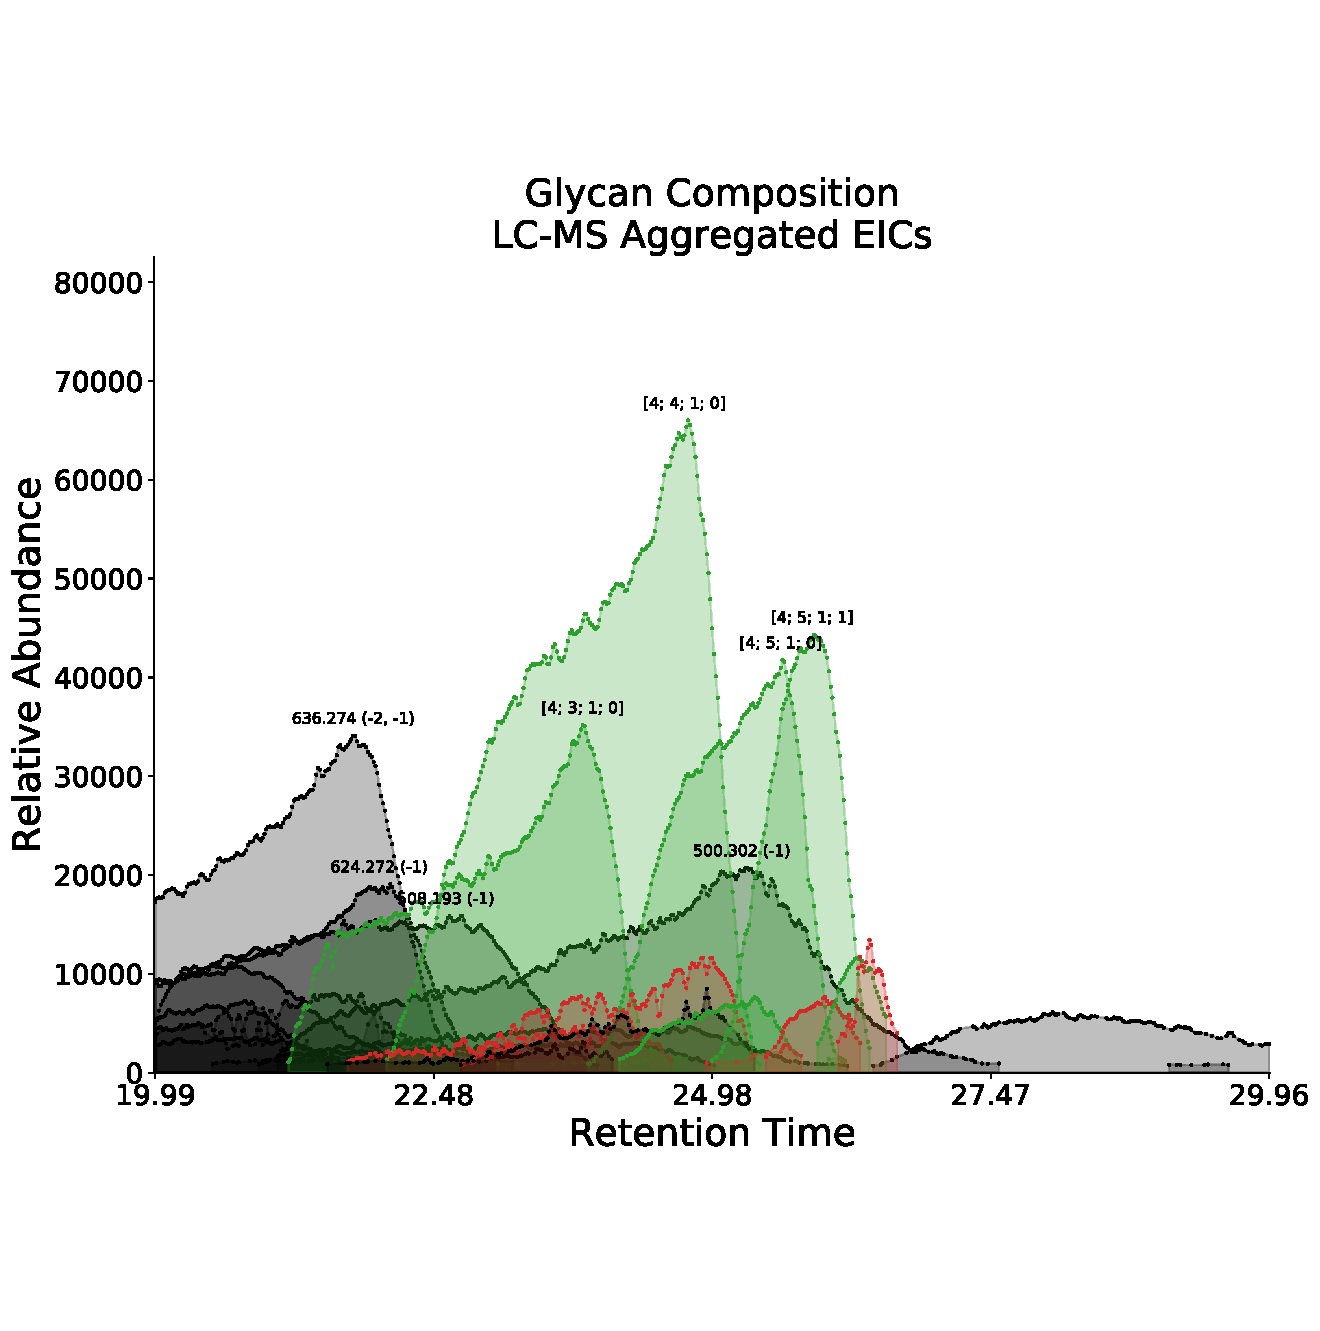
\includegraphics[width=0.45\textwidth,valign=t]{figure/igg_chromatograms.pdf}
        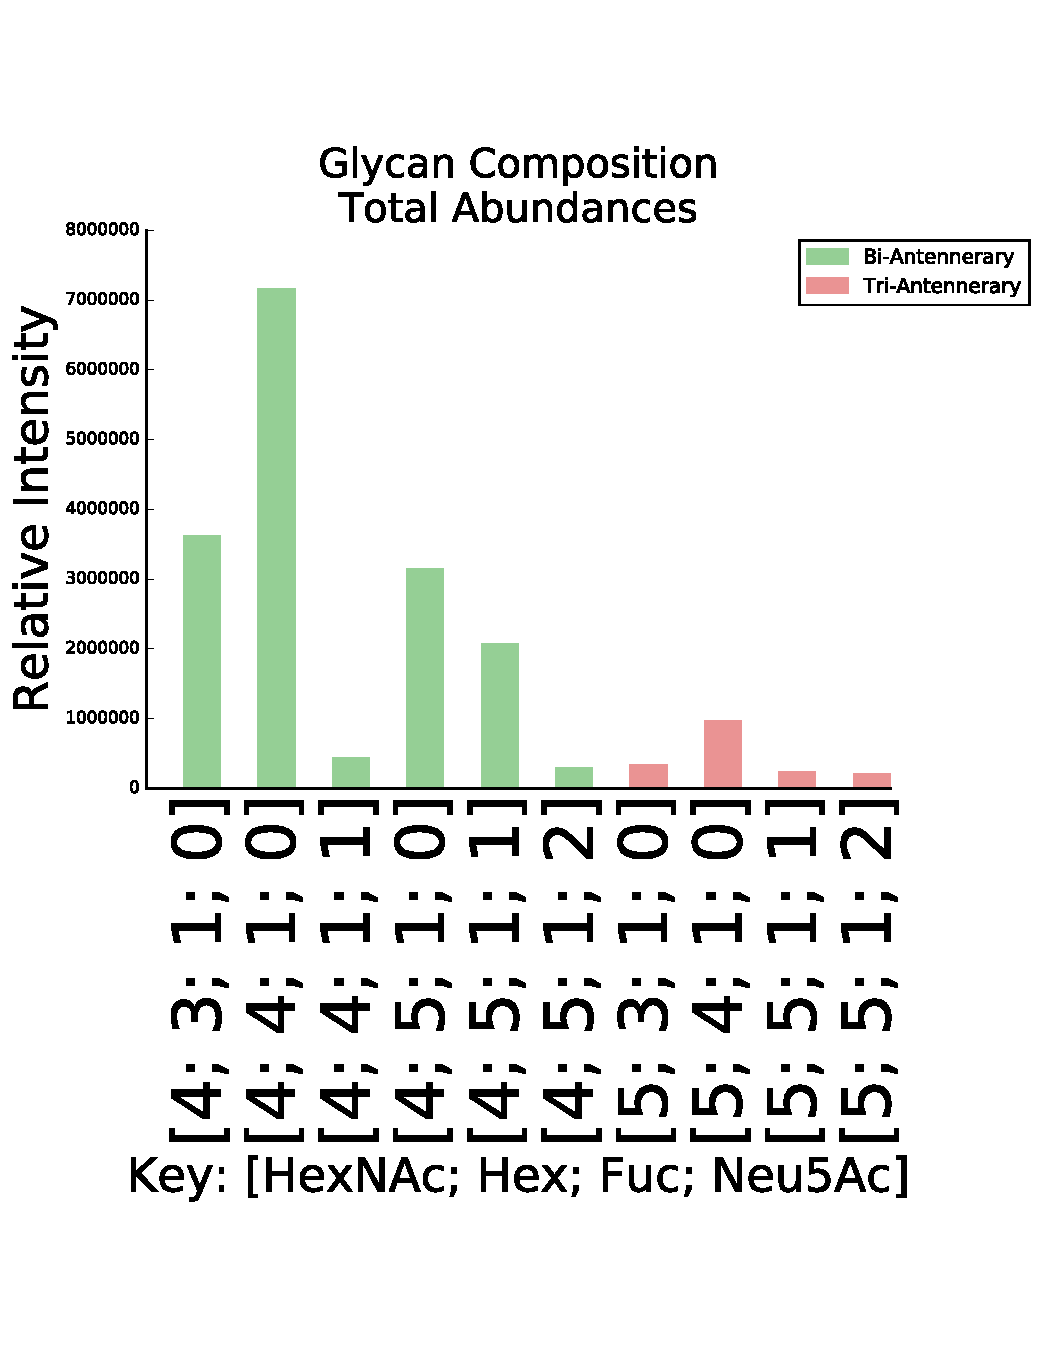
\includegraphics[width=0.45\textwidth,valign=t]{figure/igg_abundances.pdf}
        \caption{\textit{20151002-02-IGG} Glycan Relative Abundances}
        \label{fig:igg_aggregated_eics}
    \end{figure}

    \begin{table}
        \begin{minipage}[t]{0.25\linewidth}
            \vspace{0pt}
            (a)
            \centering
            
    \begin{tabular}{l | c}
        Group & $\tau$ \\
        \hline
        high-mannose & 0.00 \\
        hybrid & 14.58 \\
        bi-antennary & 8.67 \\
        asialo-bi-antennary & 14.47 \\
        tri-antennary & 5.30 \\
        asialo-tri-antennary & 11.61 \\
        tetra-antennary & 3.09 \\
        asialo-tetra-antennary & 0.00 \\
        penta-antennary & 0.00 \\
        asialo-penta-antennary & 0.00 \\
    \end{tabular}
    
            
        \end{minipage}
        \hspace{1cm}
        \begin{minipage}[t]{0.55\linewidth}
            \vspace{0pt}
            (b)
            \centering
            
    \begin{footnotesize}
    \begin{tabular}{l|p{2cm} p{2cm}}
Glycan Compostion &  Unregularized Score &  Regularized Score \\
\hline
\{Fuc:1; Hex:3; HexNAc:4\}           &                15.51 &              14.77 \\
\{Fuc:1; Hex:4; HexNAc:4\}           &                18.95 &              14.66 \\
\{Fuc:1; Hex:4; HexNAc:4; Neu5Ac:1\} &                13.23 &              12.23 \\
\{Fuc:1; Hex:5; HexNAc:4\}           &                18.23 &              14.52 \\
\{Fuc:1; Hex:5; HexNAc:4; Neu5Ac:1\} &                14.11 &              12.29 \\
\{Fuc:1; Hex:5; HexNAc:4; Neu5Ac:2\} &                11.78 &              10.95 \\
\{Fuc:1; Hex:3; HexNAc:5\}           &                11.41 &              14.15 \\
\{Fuc:1; Hex:4; HexNAc:5\}           &                15.34 &              13.57 \\
\{Fuc:1; Hex:5; HexNAc:5; Neu5Ac:1\} &                10.30 &               8.80 \\
\{Fuc:1; Hex:5; HexNAc:5; Neu5Ac:2\} &                14.07 &               7.54 \\
\end{tabular}

    \end{footnotesize}
    
        \end{minipage}
        \caption{
                 Search Results for \textit{20151002-02-IGG}.
                 (a) Estimated $\mathbf{\tau}$ for grid with ${\hat \gamma} = 13.295275$.
                 (b) Scores For Identified Glycans of grid with ${\hat \lambda} = 0.99$.}
        \label{tbl:igg_score_table}
    \end{table}

        \begin{figure}[!htbp]
        \centering
        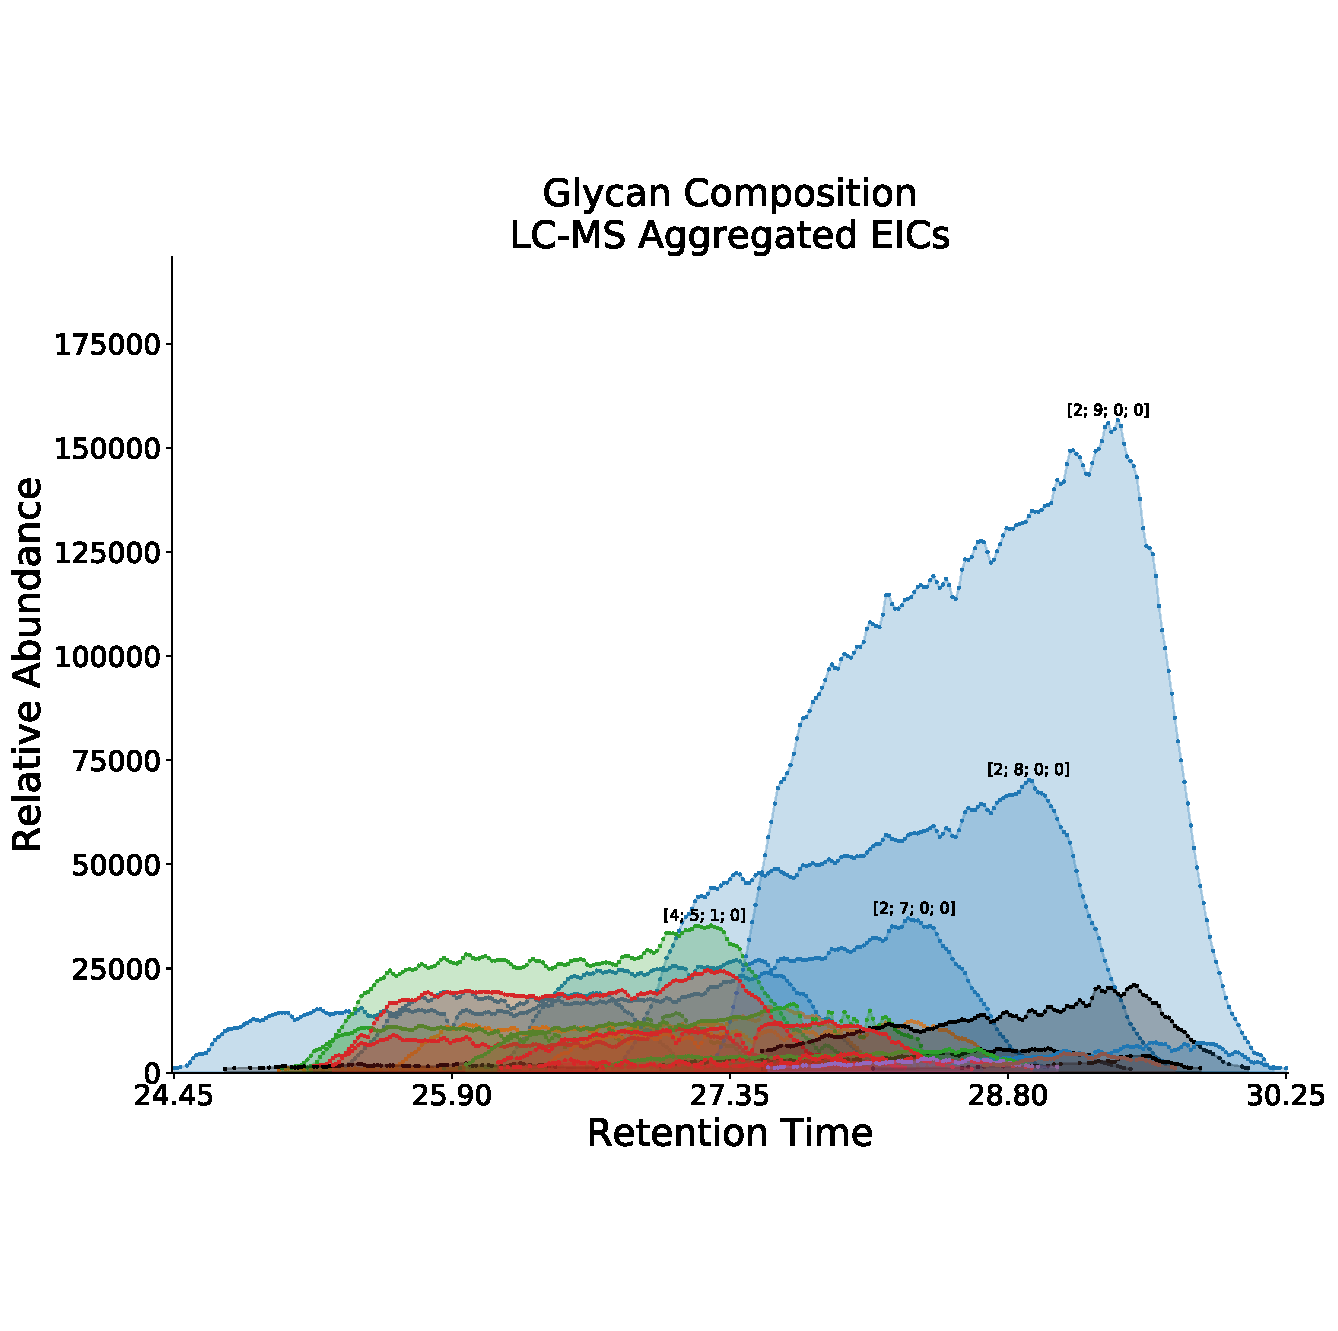
\includegraphics[width=0.45\textwidth,valign=t]{figure/phil_82_chromatograms.pdf}
        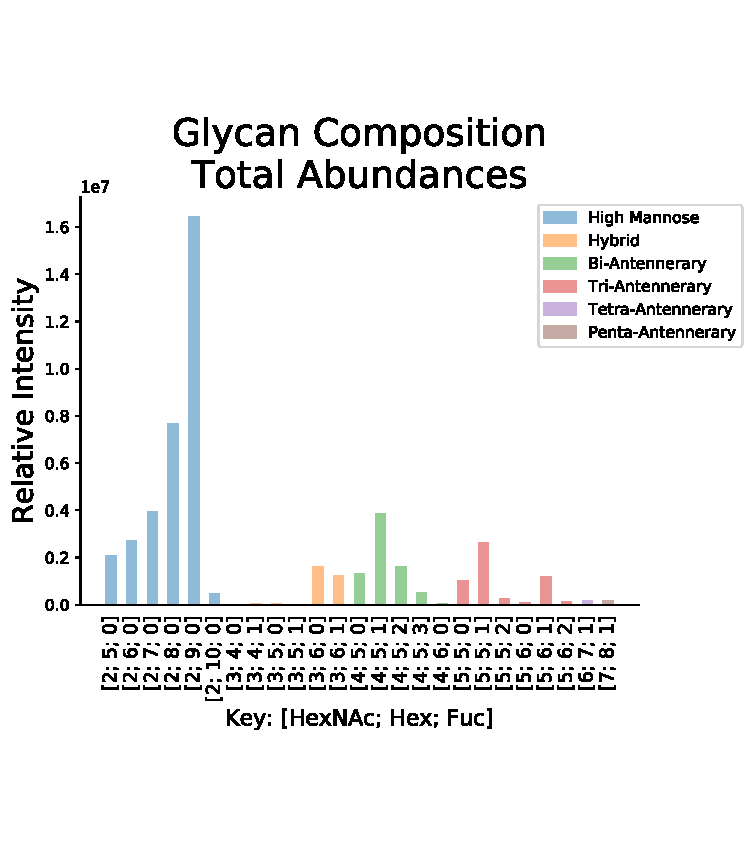
\includegraphics[width=0.45\textwidth,valign=t]{figure/phil_82_abundances.pdf}
        \caption{\textit{20141031-07-Phil-82} Glycan Relative Abundances}
        \label{fig:phil_82_aggregated_eics}
    \end{figure}

    \begin{table}
        \begin{minipage}[t]{0.25\linewidth}
            \vspace{0pt}
            (a)
            \centering
            
    \begin{tabular}{l | c}
        Group & $\tau$ \\
        \hline
        high-mannose & 15.88 \\
        hybrid & 12.12 \\
        bi-antennary & 0.00 \\
        asialo-bi-antennary & 18.57 \\
        tri-antennary & 0.00 \\
        asialo-tri-antennary & 11.61 \\
        tetra-antennary & 0.00 \\
        asialo-tetra-antennary & 6.18 \\
        penta-antennary & 0.00 \\
        asialo-penta-antennary & 0.00 \\
    \end{tabular}
    
            
        \end{minipage}
        \hspace{1cm}
        \begin{minipage}[t]{0.55\linewidth}
            \vspace{0pt}
            (b)
            \centering
            
    \begin{footnotesize}
    \begin{tabular}{l|p{2cm} p{2cm}}
Glycan Compostion &  Unregularized Score &  Regularized Score \\
\hline
\{Hex:5; HexNAc:2\}           &                14.89 &              15.23 \\
\{Hex:6; HexNAc:2\}           &                16.81 &              15.77 \\
\{Hex:7; HexNAc:2\}           &                17.27 &              16.33 \\
\{Hex:8; HexNAc:2\}           &                18.63 &              16.52 \\
\{Hex:9; HexNAc:2\}           &                19.10 &              16.20 \\
\{Hex:10; HexNAc:2\}          &                 6.80 &              13.94 \\
\{Hex:5; HexNAc:3\}           &                10.01 &              14.31 \\
\{Hex:6; HexNAc:3\}           &                17.03 &              15.17 \\
\{Fuc:1; Hex:6; HexNAc:3\}    &                16.76 &              15.20 \\
\{Hex:5; HexNAc:4\}           &                16.29 &              14.46 \\
\{Fuc:1; Hex:5; HexNAc:4\}    &                17.07 &              14.60 \\
\{Fuc:2; Hex:5; HexNAc:4\}    &                14.69 &              14.15 \\
\{Fuc:3; Hex:5; HexNAc:4\}    &                 7.75 &              13.12 \\
\{Hex:6; HexNAc:4\}           &                12.66 &              13.88 \\
\{Hex:5; HexNAc:5\}           &                16.43 &              13.35 \\
\{Fuc:1; Hex:5; HexNAc:5\}    &                16.51 &              13.36 \\
\{Hex:6; HexNAc:5\}           &                 6.74 &              11.68 \\
\{Fuc:1; Hex:6; HexNAc:5\}    &                10.94 &              12.15 \\
\{Fuc:2; Hex:6; HexNAc:5\}    &                 7.94 &              11.79 \\
\{Hex:7; HexNAc:6; Neu5Ac:4\} &                 6.39 &               1.06 \\
\{Fuc:1; Hex:7; HexNAc:6\}    &                 4.62 &               5.74 \\
\{Fuc:1; Hex:8; HexNAc:7\}    &                 8.16 &               3.49 \\
\end{tabular}

    \end{footnotesize}
    
        \end{minipage}
        \caption{
                 Search Results for \textit{20141031-07-Phil-82}.
                 (a) Estimated $\mathbf{\tau}$ for grid with ${\hat \gamma} = 15.372934$.
                 (b) Scores For Identified Glycans of grid with ${\hat \lambda} = 0.99$.}
        \label{tbl:phil_82_score_table}
    \end{table}

        \begin{figure}[!htbp]
        \centering
        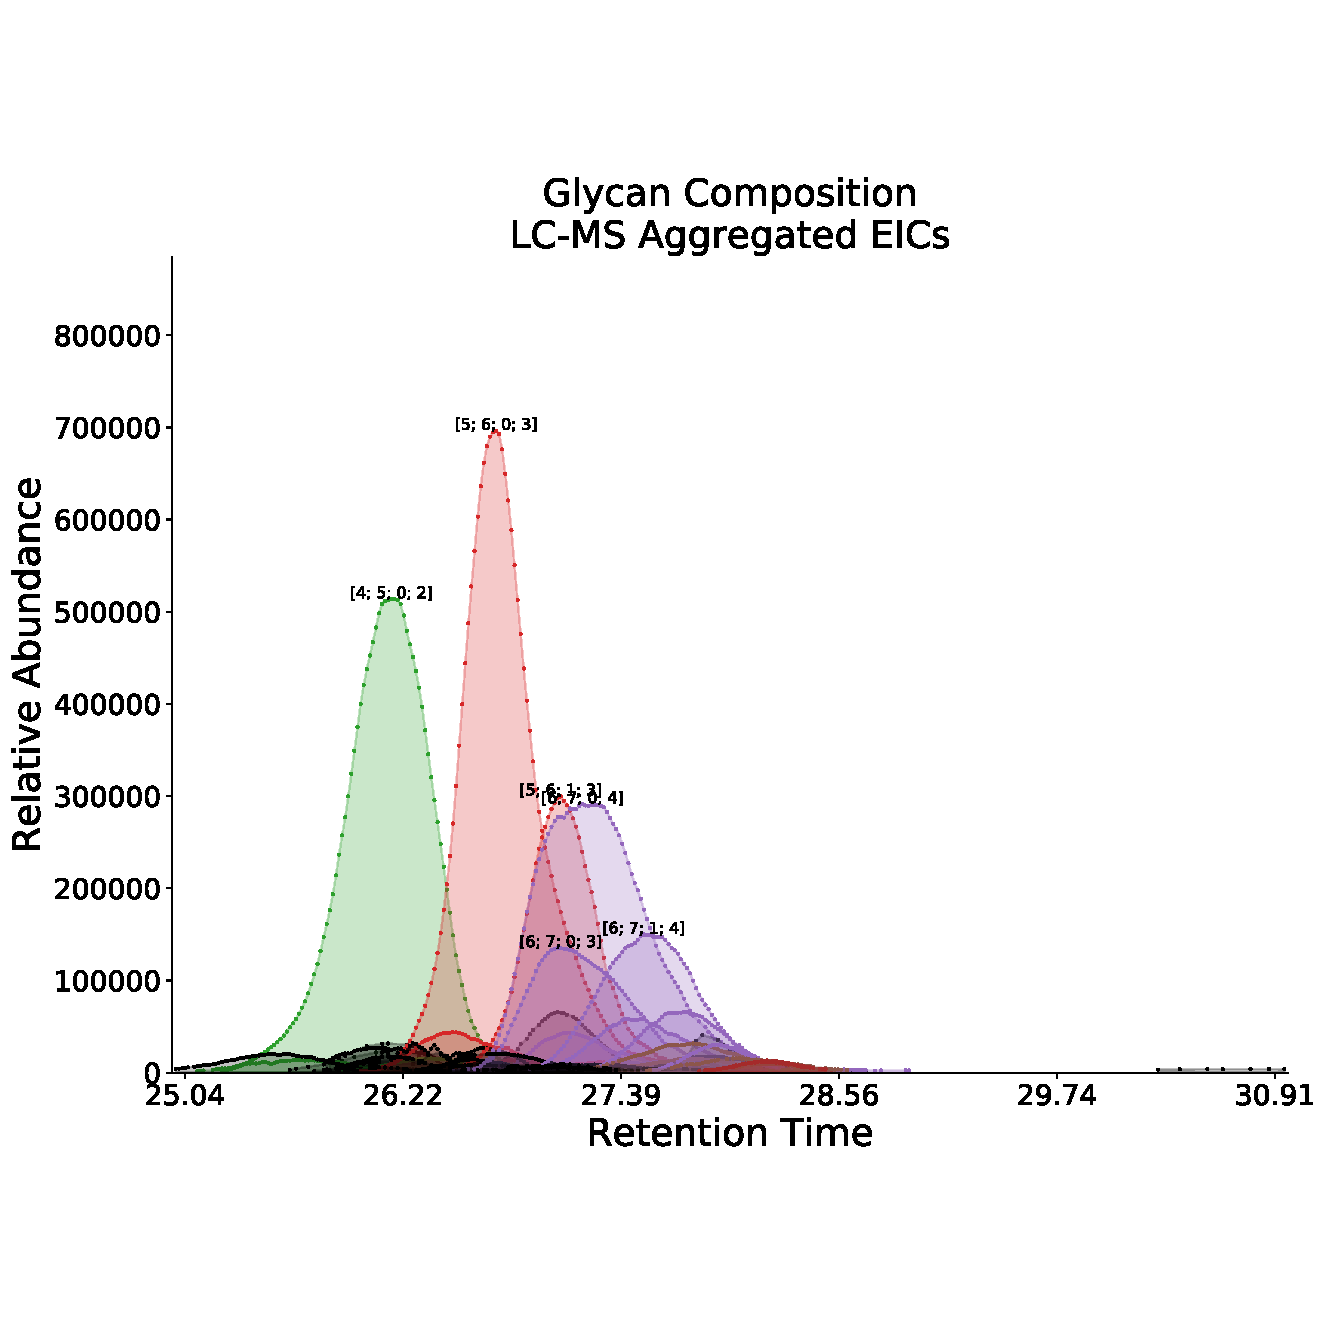
\includegraphics[width=0.45\textwidth,valign=t]{figure/agp_chromatograms.pdf}
        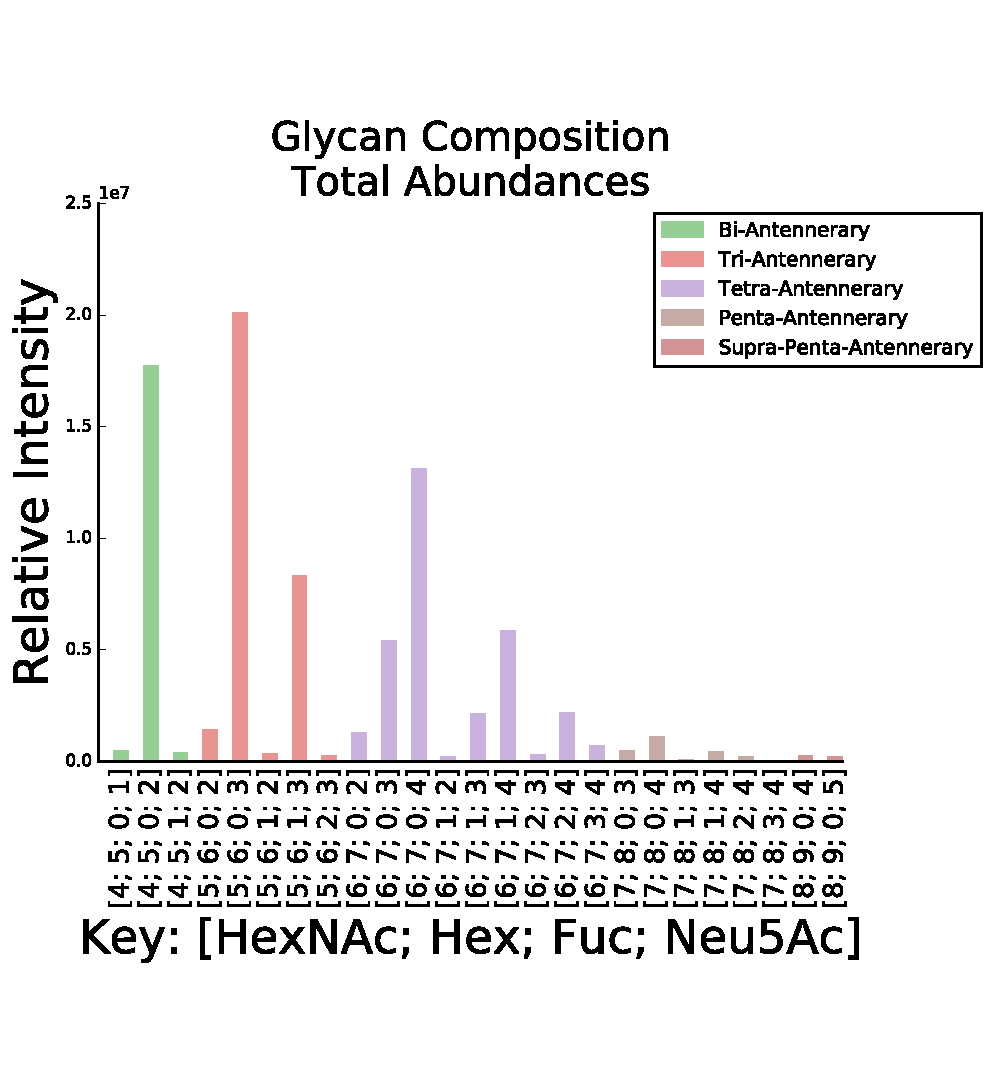
\includegraphics[width=0.45\textwidth,valign=t]{figure/agp_abundances.pdf}
        \caption{\textit{20150930-06-AGP} Glycan Relative Abundances}
        \label{fig:agp_aggregated_eics}
    \end{figure}

    \begin{table}
        \begin{minipage}[t]{0.25\linewidth}
            \vspace{0pt}
            (a)
            \centering
            
    \begin{tabular}{l | c}
        Group & $\tau$ \\
        \hline
        high-mannose & 0.00 \\
        hybrid & 11.81 \\
        bi-antennary & 15.19 \\
        asialo-bi-antennary & 1.28 \\
        tri-antennary & 21.46 \\
        asialo-tri-antennary & 0.98 \\
        tetra-antennary & 14.01 \\
        asialo-tetra-antennary & 0.00 \\
        penta-antennary & 9.61 \\
        asialo-penta-antennary & 0.00 \\
    \end{tabular}
    
            
        \end{minipage}
        \hspace{1cm}
        \begin{minipage}[t]{0.55\linewidth}
            \vspace{0pt}
            (b)
            \centering
            
    \begin{footnotesize}
    \begin{tabular}{l|p{2cm} p{2cm}}
Glycan Compostion &  Unregularized Score &  Regularized Score \\
\hline
\{Hex:5; HexNAc:4; Neu5Ac:1\}        &                13.33 &              10.00 \\
\{Hex:5; HexNAc:4; Neu5Ac:2\}        &                23.36 &              16.47 \\
\{Fuc:1; Hex:5; HexNAc:4; Neu5Ac:2\} &                13.92 &              15.11 \\
\{Hex:6; HexNAc:5; Neu5Ac:2\}        &                19.77 &              17.49 \\
\{Hex:6; HexNAc:5; Neu5Ac:3\}        &                20.13 &              17.60 \\
\{Fuc:1; Hex:6; HexNAc:5; Neu5Ac:2\} &                17.68 &              17.12 \\
\{Fuc:1; Hex:6; HexNAc:5; Neu5Ac:3\} &                17.53 &              17.08 \\
\{Fuc:2; Hex:6; HexNAc:5; Neu5Ac:3\} &                12.97 &              16.40 \\
\{Hex:7; HexNAc:6; Neu5Ac:2\}        &                17.96 &              16.21 \\
\{Hex:7; HexNAc:6; Neu5Ac:3\}        &                17.35 &              16.18 \\
\{Hex:7; HexNAc:6; Neu5Ac:4\}        &                20.81 &              16.55 \\
\{Fuc:1; Hex:7; HexNAc:6; Neu5Ac:2\} &                12.55 &              15.59 \\
\{Fuc:1; Hex:7; HexNAc:6; Neu5Ac:3\} &                17.32 &              15.91 \\
\{Fuc:1; Hex:7; HexNAc:6; Neu5Ac:4\} &                17.17 &              15.95 \\
\{Fuc:2; Hex:7; HexNAc:6; Neu5Ac:3\} &                 8.66 &              14.98 \\
\{Fuc:2; Hex:7; HexNAc:6; Neu5Ac:4\} &                16.66 &              15.61 \\
\{Fuc:3; Hex:7; HexNAc:6; Neu5Ac:4\} &                13.77 &              15.28 \\
\{Hex:8; HexNAc:7; Neu5Ac:3\}        &                13.27 &              12.00 \\
\{Hex:8; HexNAc:7; Neu5Ac:4\}        &                12.81 &              11.97 \\
\{Fuc:1; Hex:8; HexNAc:7; Neu5Ac:3\} &                 8.78 &              11.48 \\
\{Fuc:1; Hex:8; HexNAc:7; Neu5Ac:4\} &                10.66 &              11.62 \\
\{Fuc:2; Hex:8; HexNAc:7; Neu5Ac:4\} &                 9.66 &              11.45 \\
\{Fuc:3; Hex:8; HexNAc:7; Neu5Ac:4\} &                 7.59 &              11.25 \\
\{Hex:9; HexNAc:8; Neu5Ac:4\}        &                11.12 &               9.80 \\
\{Hex:9; HexNAc:8; Neu5Ac:5\}        &                 9.15 &               9.58 \\
\end{tabular}

    \end{footnotesize}
    
        \end{minipage}
        \caption{
                 Search Results for \textit{20150930-06-AGP}.
                 (a) Estimated $\mathbf{\tau}$ for grid with ${\hat \gamma} = 14.837758$.
                 (b) Scores For Identified Glycans of grid with ${\hat \lambda} = 0.99$.}
        \label{tbl:agp_score_table}
    \end{table}

        \begin{figure}[!htbp]
        \centering
        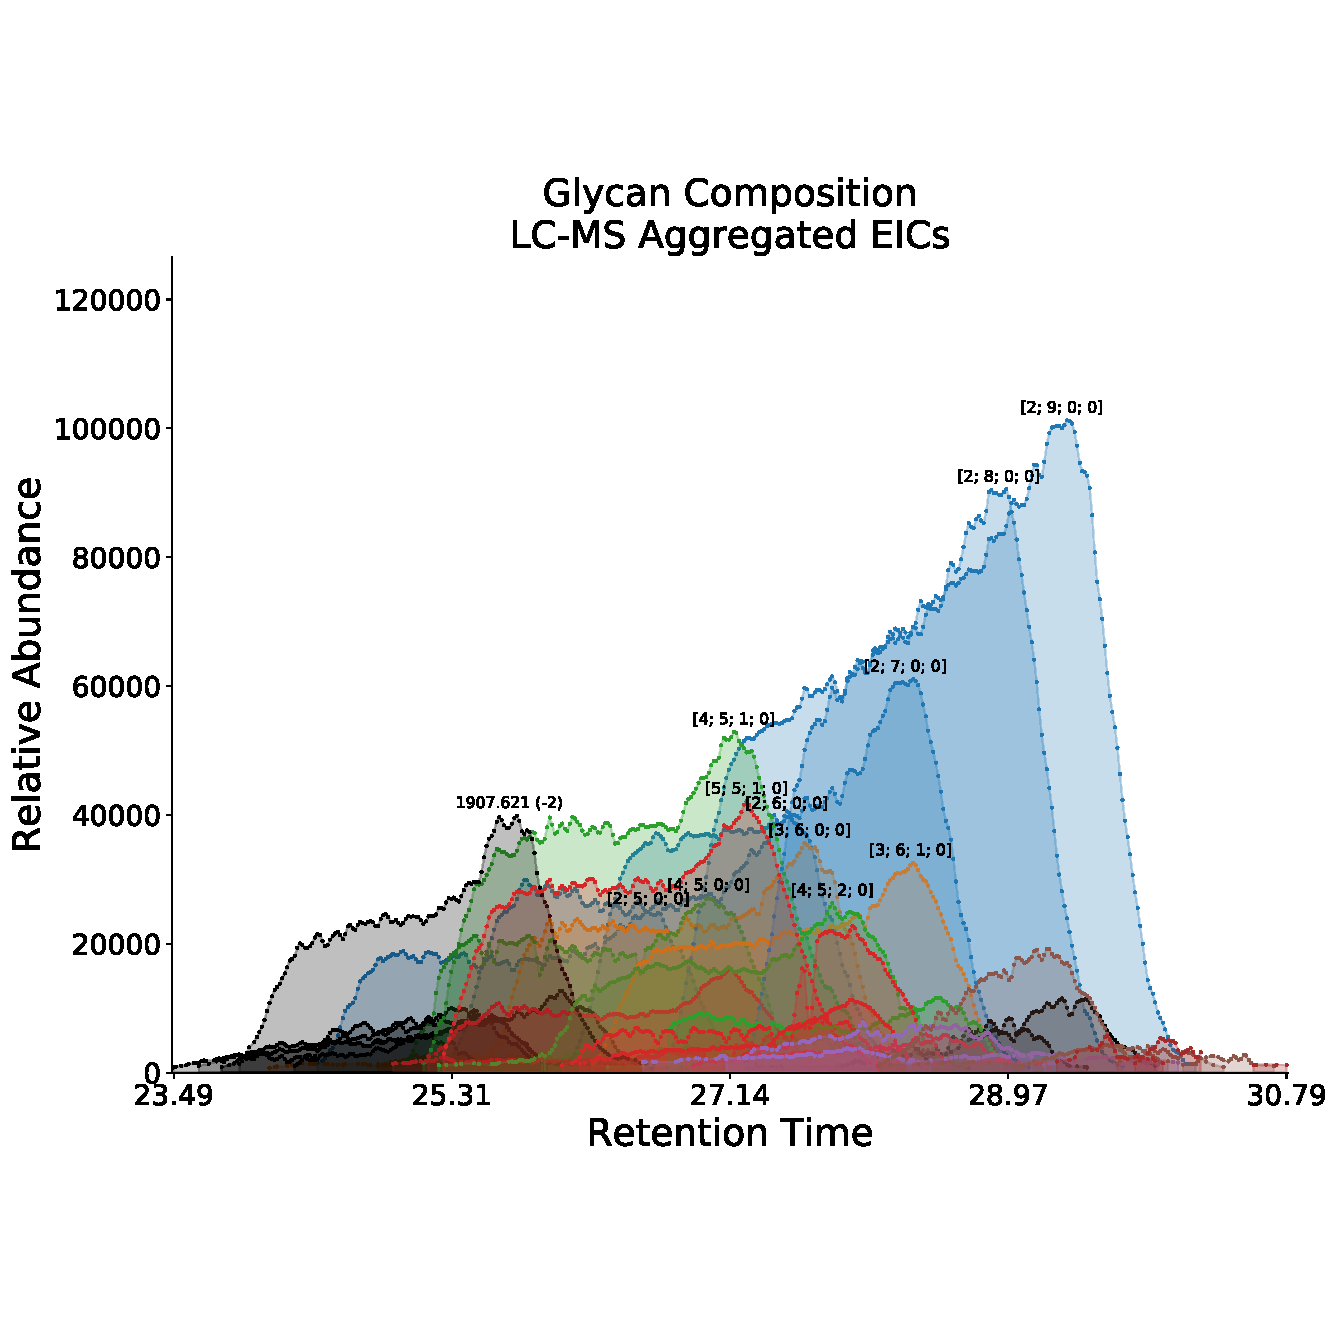
\includegraphics[width=0.45\textwidth,valign=t]{figure/phil_bs_chromatograms.pdf}
        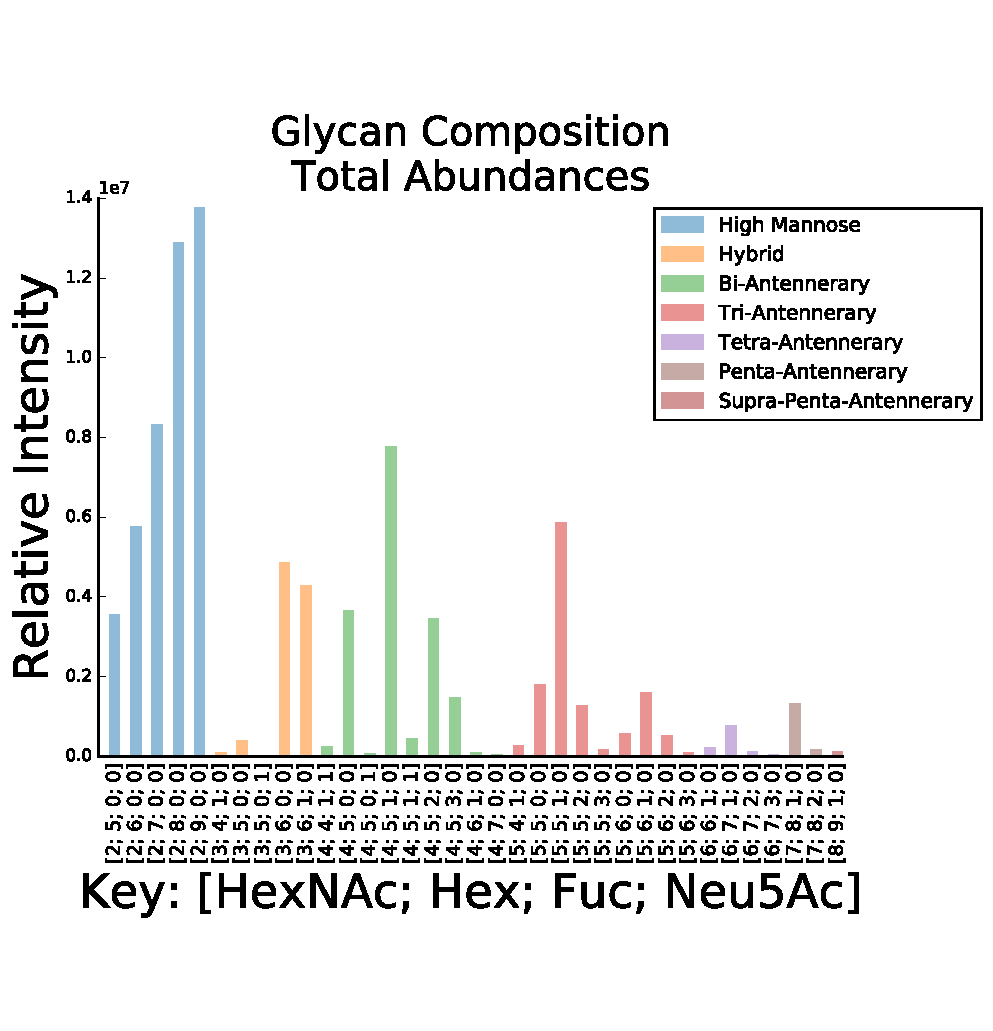
\includegraphics[width=0.45\textwidth,valign=t]{figure/phil_bs_abundances.pdf}
        \caption{\textit{20141101-04-Phil-BS} Glycan Relative Abundances}
        \label{fig:phil_bs_aggregated_eics}
    \end{figure}

    \begin{table}
        \begin{minipage}[t]{0.25\linewidth}
            \vspace{0pt}
            (a)
            \centering
            
    \begin{tabular}{l | c}
        Group & $\tau$ \\
        \hline
        high-mannose & 1.86 \\
        hybrid & 1.50 \\
        bi-antennary & 0.00 \\
        asialo-bi-antennary & 1.70 \\
        tri-antennary & 0.00 \\
        asialo-tri-antennary & 0.94 \\
        tetra-antennary & 0.00 \\
        asialo-tetra-antennary & 0.89 \\
        penta-antennary & 0.00 \\
        asialo-penta-antennary & 0.61 \\
    \end{tabular}
    
            
        \end{minipage}
        \hspace{1cm}
        \begin{minipage}[t]{0.55\linewidth}
            \vspace{0pt}
            (b)
            \centering
            
    \begin{footnotesize}
    \begin{tabular}{l|p{2cm} p{2cm}}
Glycan Compostion &  Unregularized Score &  Regularized Score \\
\hline
\{Hex:5; HexNAc:2\}                  &                18.44 &              18.03 \\
\{Hex:6; HexNAc:2\}                  &                17.74 &              17.53 \\
\{Hex:7; HexNAc:2\}                  &                17.94 &              17.64 \\
\{Hex:8; HexNAc:2\}                  &                19.02 &              18.64 \\
\{Hex:9; HexNAc:2\}                  &                19.91 &              19.37 \\
\{Fuc:1; Hex:4; HexNAc:3\}           &                10.74 &              10.40 \\
\{Hex:5; HexNAc:3\}                  &                11.95 &              11.90 \\
\{Hex:5; HexNAc:3; Neu5Ac:1\}        &                 7.71 &               7.68 \\
\{Hex:6; HexNAc:3\}                  &                19.15 &              18.62 \\
\{Fuc:1; Hex:6; HexNAc:3\}           &                17.20 &              16.62 \\
\{Hex:7; HexNAc:3; Neu5Ac:1\}        &                 8.19 &               7.98 \\
\{Fuc:1; Hex:4; HexNAc:4; Neu5Ac:1\} &                 9.02 &               8.66 \\
\{Hex:5; HexNAc:4\}                  &                15.62 &              15.31 \\
\{Hex:5; HexNAc:4; Neu5Ac:1\}        &                11.41 &              11.05 \\
\{Fuc:1; Hex:5; HexNAc:4\}           &                17.64 &              17.15 \\
\{Fuc:1; Hex:5; HexNAc:4; Neu5Ac:1\} &                 7.95 &               7.87 \\
\{Fuc:2; Hex:5; HexNAc:4\}           &                16.33 &              15.72 \\
\{Fuc:3; Hex:5; HexNAc:4\}           &                11.08 &              10.83 \\
\{Fuc:1; Hex:6; HexNAc:4\}           &                12.31 &              12.11 \\
\{Hex:7; HexNAc:4\}                  &                11.97 &              11.58 \\
\{Hex:8; HexNAc:4; Neu5Ac:2\}        &                 6.75 &               6.50 \\
\{Fuc:1; Hex:4; HexNAc:5\}           &                12.16 &              11.74 \\
\{Hex:5; HexNAc:5\}                  &                17.18 &              16.63 \\
\{Fuc:1; Hex:5; HexNAc:5\}           &                17.37 &              16.80 \\
\{Fuc:2; Hex:5; HexNAc:5\}           &                 8.08 &               8.06 \\
\{Fuc:3; Hex:5; HexNAc:5\}           &                 7.51 &               7.33 \\
\{Hex:6; HexNAc:5\}                  &                10.03 &               9.89 \\
\{Fuc:1; Hex:6; HexNAc:5\}           &                11.89 &              11.63 \\
\{Fuc:2; Hex:6; HexNAc:5\}           &                 8.99 &               8.78 \\
\{Fuc:3; Hex:6; HexNAc:5\}           &                 8.19 &               7.92 \\
\{Hex:9; HexNAc:5; Neu5Ac:2\}        &                11.40 &              10.72 \\
\{Fuc:1; Hex:6; HexNAc:6\}           &                 7.79 &               7.59 \\
\{Fuc:1; Hex:7; HexNAc:6\}           &                 9.13 &               8.81 \\
\{Fuc:2; Hex:7; HexNAc:6\}           &                 7.39 &               7.20 \\
\{Fuc:3; Hex:7; HexNAc:6\}           &                 7.46 &               7.15 \\
\{Fuc:1; Hex:8; HexNAc:7\}           &                17.25 &              16.39 \\
\{Fuc:2; Hex:8; HexNAc:7\}           &                15.20 &              14.46 \\
\{Hex:3; HexNAc:8; Neu5Ac:4\}        &                10.11 &               9.56 \\
\{Fuc:1; Hex:9; HexNAc:8\}           &                13.44 &              12.70 \\
\end{tabular}

    \end{footnotesize}
    
        \end{minipage}
        \caption{
                 Search Results for \textit{20141101-04-Phil-BS}.
                 (a) Estimated $\mathbf{\tau}$ for grid with ${\hat \gamma} = 15.74699$.
                 (b) Scores For Identified Glycans of grid with ${\hat \lambda} = 0.01$.}
        \label{tbl:phil_bs_score_table}
    \end{table}



\subsection{Deuteroreduced and Permethylated N-Glycans}
    The results for \textit{20141128-11-Phil-82} are shown in Table \ref{tbl:dp_phil_82_score_table}
    and visualized in Figure \ref{fig:dp_phil_82_aggregated_eics}. The results for \textit{AGP-DR-Perm-glycans-1}
    are shown in Table \ref{tbl:dp_agp_score_table} and visualized in Figure \ref{fig:dp_agp_aggregated_eics}.

        \begin{figure}[!htbp]
        \centering
        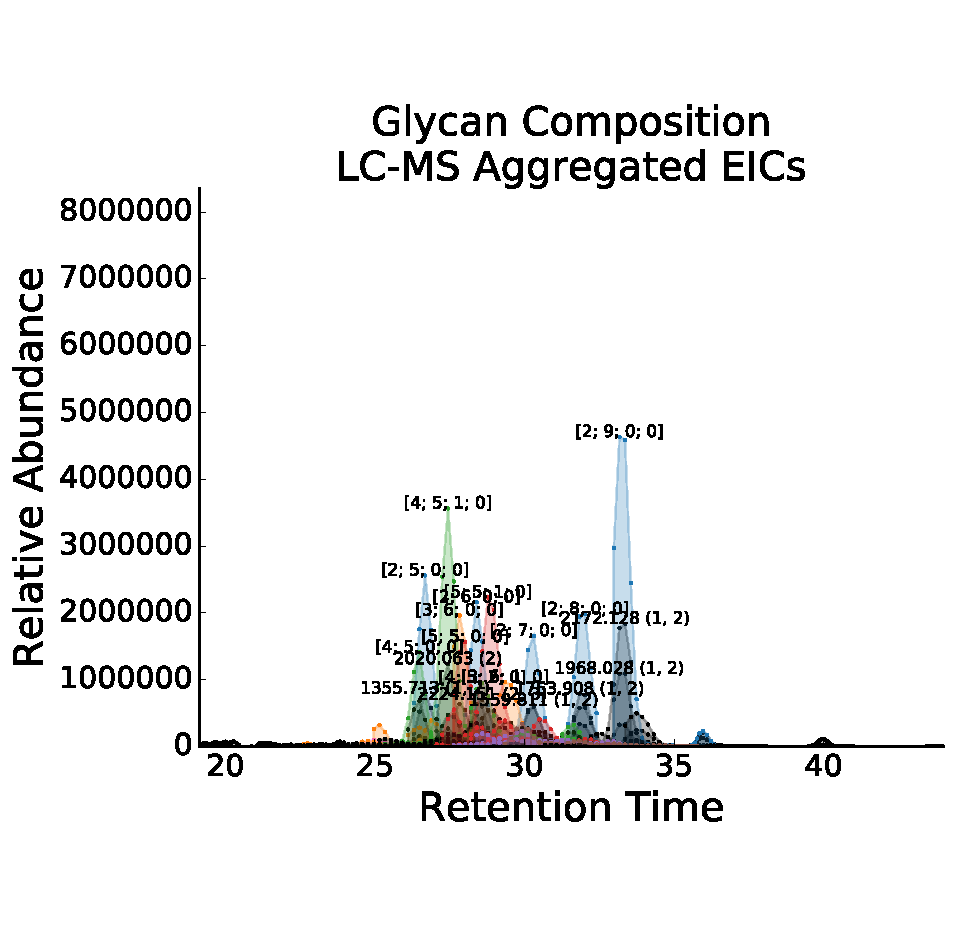
\includegraphics[width=0.45\textwidth,valign=t]{figure/dp_phil_82_chromatograms.pdf}
        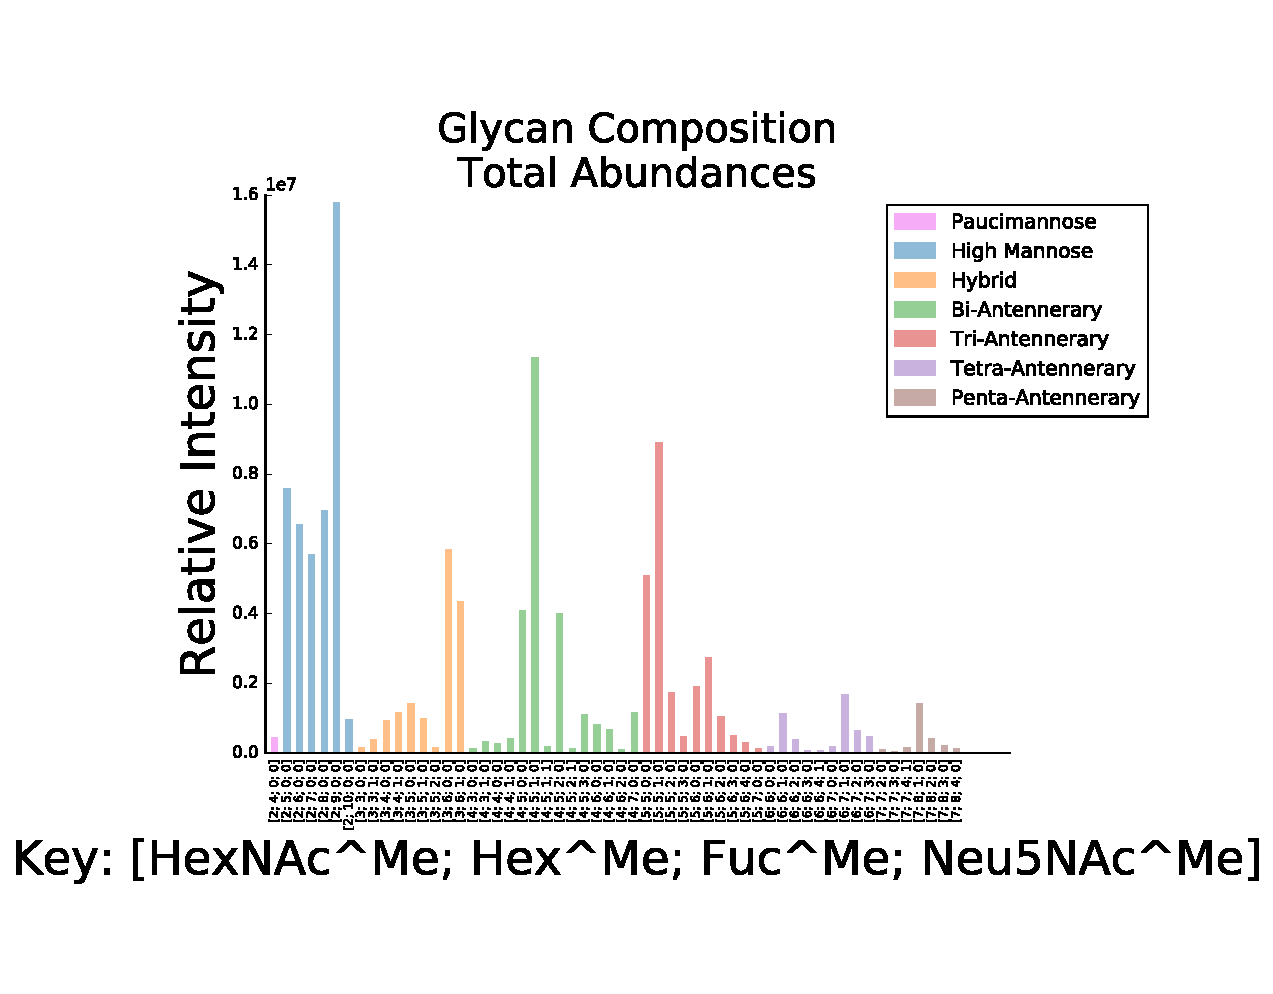
\includegraphics[width=0.45\textwidth,valign=t]{figure/dp_phil_82_abundances.pdf}
        \caption{\textit{20141128-11-Phil-82} Glycan Relative Abundances}
        \label{fig:dp_phil_82_aggregated_eics}
    \end{figure}

    \begin{table}
        \begin{minipage}[t]{0.25\linewidth}
            \vspace{0pt}
            (a)
            \centering
            
    \begin{tabular}{l | c}
        Group & $\tau$ \\
        \hline
        high-mannose & 18.08 \\
        hybrid & 15.20 \\
        bi-antennary & 1.42 \\
        asialo-bi-antennary & 21.55 \\
        tri-antennary & 0.74 \\
        asialo-tri-antennary & 17.12 \\
        tetra-antennary & 0.00 \\
        asialo-tetra-antennary & 10.61 \\
        penta-antennary & 0.00 \\
        asialo-penta-antennary & 2.91 \\
    \end{tabular}
    
            
        \end{minipage}
        \hspace{1cm}
        \begin{minipage}[t]{0.55\linewidth}
            \vspace{0pt}
            (b)
            \centering
            
    \begin{footnotesize}
    \begin{tabular}{l|p{2cm} p{2cm}}
Glycan Compostion &  Unregularized Score &  Regularized Score \\
\hline
\{Hex:4; HexNAc:2\}                   &                17.40 &              17.64 \\
\{Hex:5; HexNAc:2\}                   &                20.14 &              18.28 \\
\{Hex:6; HexNAc:2\}                   &                22.02 &              18.71 \\
\{Hex:7; HexNAc:2\}                   &                21.78 &              19.01 \\
\{Hex:8; HexNAc:2\}                   &                15.52 &              17.70 \\
\{Hex:9; HexNAc:2\}                   &                16.43 &              17.43 \\
\{Hex:10; HexNAc:2\}                  &                12.24 &              16.62 \\
\{Hex:3; HexNAc:3\}                   &                15.09 &              17.25 \\
\{Fuc:1; Hex:3; HexNAc:3\}            &                19.38 &              17.99 \\
\{Hex:4; HexNAc:3\}                   &                17.48 &              17.65 \\
\{Fuc:1; Hex:4; HexNAc:3\}            &                20.29 &              18.07 \\
\{Hex:5; HexNAc:3\}                   &                17.18 &              17.86 \\
\{Fuc:1; Hex:5; HexNAc:3\}            &                20.16 &              18.15 \\
\{Fuc:2; Hex:5; HexNAc:3\}            &                12.93 &              17.21 \\
\{Hex:6; HexNAc:3\}                   &                15.06 &              17.76 \\
\{Fuc:1; Hex:6; HexNAc:3\}            &                16.30 &              17.72 \\
\{Hex:7; HexNAc:3\}                   &                 6.85 &               1.02 \\
\{Hex:3; HexNAc:4\}                   &                11.87 &              16.82 \\
\{Fuc:1; Hex:3; HexNAc:4\}            &                17.49 &              17.69 \\
\{Hex:4; HexNAc:4\}                   &                13.19 &              16.88 \\
\{Fuc:1; Hex:4; HexNAc:4\}            &                 9.31 &              16.76 \\
\{Hex:5; HexNAc:4\}                   &                17.27 &              17.72 \\
\{Fuc:1; Hex:5; HexNAc:4\}            &                21.31 &              18.21 \\
\{Fuc:1; Hex:5; HexNAc:4; Neu5NAc:1\} &                16.43 &              12.93 \\
\{Fuc:2; Hex:5; HexNAc:4\}            &                21.10 &              18.01 \\
\{Fuc:2; Hex:5; HexNAc:4; Neu5NAc:1\} &                 6.09 &              11.83 \\
\{Fuc:3; Hex:5; HexNAc:4\}            &                19.42 &              18.07 \\
\{Hex:6; HexNAc:4\}                   &                16.30 &              17.59 \\
\{Fuc:1; Hex:6; HexNAc:4\}            &                16.56 &              17.54 \\
\{Fuc:2; Hex:6; HexNAc:4\}            &                 7.00 &              16.46 \\
\{Hex:7; HexNAc:4\}                   &                17.23 &              17.26 \\
\{Hex:5; HexNAc:5\}                   &                20.42 &              17.62 \\
\{Fuc:1; Hex:5; HexNAc:5\}            &                20.33 &              17.67 \\
\{Fuc:2; Hex:5; HexNAc:5\}            &                20.81 &              17.55 \\
\{Fuc:3; Hex:5; HexNAc:5\}            &                16.31 &              16.89 \\
\{Hex:6; HexNAc:5\}                   &                16.75 &              16.90 \\
\{Fuc:1; Hex:6; HexNAc:5\}            &                16.93 &              16.93 \\
\{Fuc:2; Hex:6; HexNAc:5\}            &                16.08 &              16.54 \\
\{Fuc:3; Hex:6; HexNAc:5\}            &                15.51 &              16.21 \\
\{Fuc:4; Hex:6; HexNAc:5\}            &                11.44 &              15.58 \\
\{Hex:7; HexNAc:5\}                   &                14.13 &              14.08 \\
\{Fuc:2; Hex:4; HexNAc:6; Neu5NAc:3\} &                 6.53 &               1.47 \\
\{Fuc:3; Hex:5; HexNAc:6; Neu5NAc:2\} &                 6.52 &               1.20 \\
\{Hex:6; HexNAc:6\}                   &                12.92 &              11.18 \\
\{Fuc:1; Hex:6; HexNAc:6\}            &                17.39 &              11.71 \\
\{Fuc:2; Hex:6; HexNAc:6\}            &                13.64 &              11.07 \\
\{Fuc:3; Hex:6; HexNAc:6\}            &                 4.15 &               9.80 \\
\{Fuc:4; Hex:6; HexNAc:6; Neu5NAc:1\} &                 6.51 &               6.96 \\
\{Hex:7; HexNAc:6\}                   &                10.41 &              10.46 \\
\{Fuc:1; Hex:7; HexNAc:6\}            &                14.80 &              10.98 \\
\{Fuc:2; Hex:7; HexNAc:6\}            &                12.54 &              10.55 \\
\{Fuc:3; Hex:7; HexNAc:6\}            &                 7.90 &               9.82 \\
\{Fuc:2; Hex:5; HexNAc:7; Neu5NAc:3\} &                 8.58 &               1.04 \\
\{Fuc:3; Hex:6; HexNAc:7; Neu5NAc:2\} &                 8.57 &               1.03 \\
\{Fuc:2; Hex:7; HexNAc:7\}            &                 4.18 &               6.48 \\
\{Fuc:3; Hex:7; HexNAc:7\}            &                 5.15 &               6.51 \\
\{Fuc:4; Hex:7; HexNAc:7; Neu5NAc:1\} &                 8.56 &               5.14 \\
\{Fuc:1; Hex:8; HexNAc:7\}            &                11.57 &               7.24 \\
\{Fuc:2; Hex:8; HexNAc:7\}            &                 9.62 &               7.00 \\
\{Fuc:3; Hex:8; HexNAc:7\}            &                10.53 &               7.11 \\
\{Fuc:4; Hex:8; HexNAc:7\}            &                12.60 &               7.43 \\
\{Hex:9; HexNAc:7\}                   &                10.32 &               4.05 \\
\end{tabular}

    \end{footnotesize}
    
        \end{minipage}
        \caption{
                 Search Results for \textit{20141128-11-Phil-82}.
                 (a) Estimated $\mathbf{\tau}$ for grid with ${\hat \gamma} = 17.653258$.
                 (b) Scores For Identified Glycans of grid with ${\hat \lambda} = 0.99$.}
        \label{tbl:dp_phil_82_score_table}
    \end{table}

        \begin{figure}[!htbp]
        \centering
        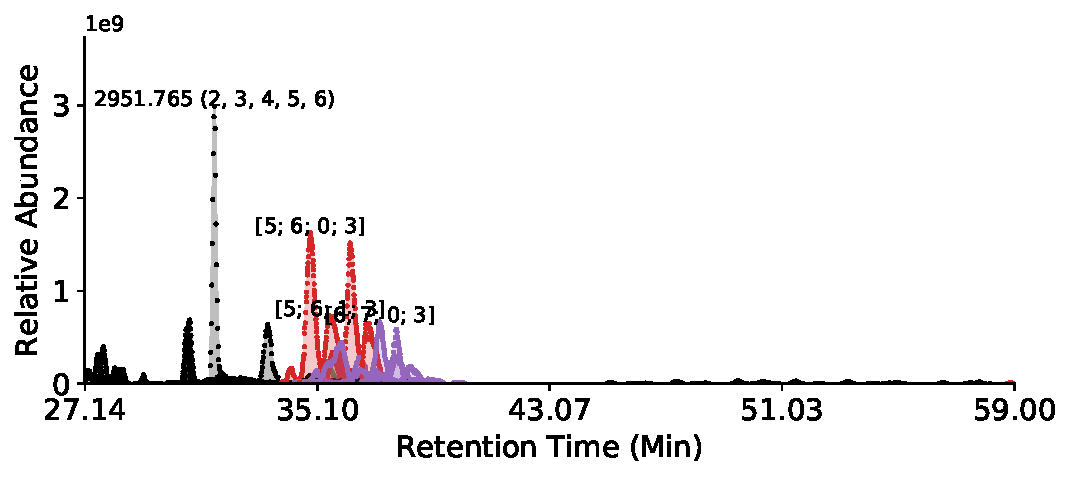
\includegraphics[width=0.45\textwidth,valign=t]{figure/dp_agp_chromatograms.pdf}
        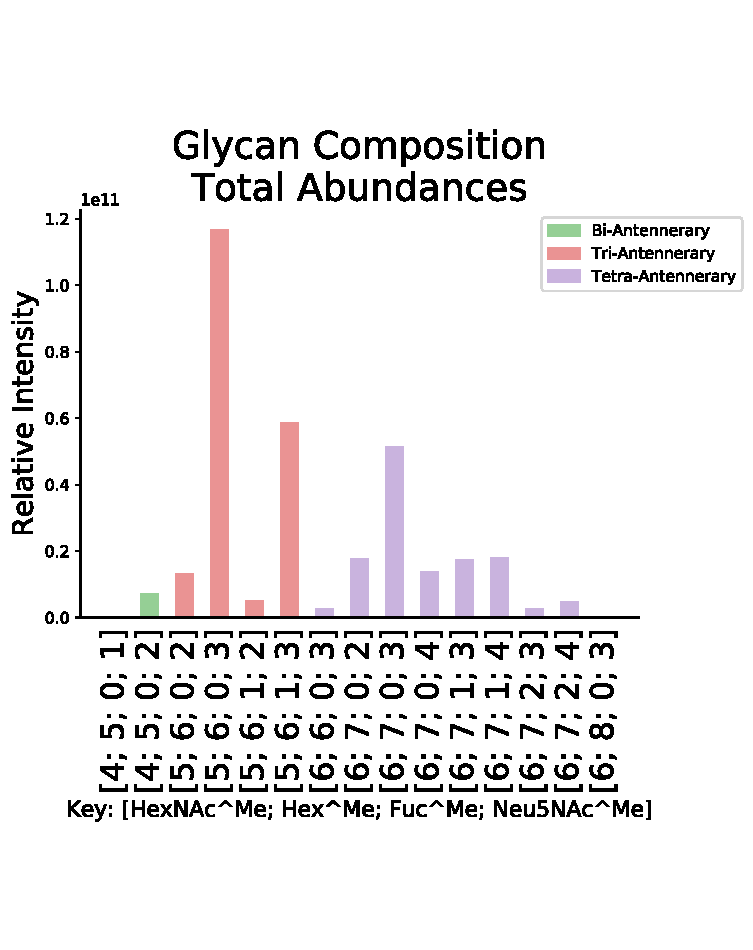
\includegraphics[width=0.45\textwidth,valign=t]{figure/dp_agp_abundances.pdf}
        \caption{\textit{AGP-DR-Perm-glycans-1} Glycan Relative Abundances}
        \label{fig:dp_agp_aggregated_eics}
    \end{figure}

    \begin{table}
        \begin{minipage}[t]{0.25\linewidth}
            \vspace{0pt}
            (a)
            \centering
            
    \begin{tabular}{l | c}
        Group & $\tau$ \\
        \hline
        high-mannose & 0.00 \\
        hybrid & 7.67 \\
        bi-antennary & 15.20 \\
        asialo-bi-antennary & 0.00 \\
        tri-antennary & 22.11 \\
        asialo-tri-antennary & 0.00 \\
        tetra-antennary & 14.57 \\
        asialo-tetra-antennary & 0.00 \\
        penta-antennary & 8.22 \\
        asialo-penta-antennary & 0.00 \\
    \end{tabular}
    
            
        \end{minipage}
        \hspace{1cm}
        \begin{minipage}[t]{0.55\linewidth}
            \vspace{0pt}
            (b)
            \centering
            
    \begin{footnotesize}
    \begin{tabular}{l|p{2cm} p{2cm}}
Glycan Compostion &  Unregularized Score &  Regularized Score \\
\hline
\{Hex:5; HexNAc:4; Neu5NAc:2\}        &                18.73 &              13.71 \\
\{Fuc:1; Hex:5; HexNAc:4; Neu5NAc:2\} &                 4.28 &              11.87 \\
\{Hex:5; HexNAc:5; Neu5NAc:2\}        &                 9.36 &              16.09 \\
\{Fuc:1; Hex:5; HexNAc:5; Neu5NAc:2\} &                 6.60 &              15.61 \\
\{Hex:6; HexNAc:5; Neu5NAc:2\}        &                18.70 &              17.12 \\
\{Hex:6; HexNAc:5; Neu5NAc:3\}        &                20.89 &              17.53 \\
\{Fuc:1; Hex:6; HexNAc:5; Neu5NAc:2\} &                 8.45 &              15.93 \\
\{Fuc:1; Hex:6; HexNAc:5; Neu5NAc:3\} &                19.75 &              17.33 \\
\{Hex:7; HexNAc:5; Neu5NAc:3\}        &                 8.29 &              17.20 \\
\{Hex:7; HexNAc:6; Neu5NAc:1\}        &                 8.48 &               5.81 \\
\{Hex:7; HexNAc:6; Neu5NAc:2\}        &                19.28 &              16.27 \\
\{Hex:7; HexNAc:6; Neu5NAc:3\}        &                19.70 &              16.11 \\
\{Hex:7; HexNAc:6; Neu5NAc:4\}        &                18.42 &              16.03 \\
\{Fuc:1; Hex:7; HexNAc:6; Neu5NAc:2\} &                 9.07 &              15.04 \\
\{Fuc:1; Hex:7; HexNAc:6; Neu5NAc:3\} &                14.38 &              15.45 \\
\{Fuc:1; Hex:7; HexNAc:6; Neu5NAc:4\} &                15.64 &              15.52 \\
\{Fuc:2; Hex:7; HexNAc:6; Neu5NAc:3\} &                10.21 &              15.06 \\
\{Fuc:2; Hex:7; HexNAc:6; Neu5NAc:4\} &                14.24 &              15.12 \\
\{Fuc:3; Hex:7; HexNAc:6; Neu5NAc:4\} &                 7.55 &              14.38 \\
\{Hex:8; HexNAc:7; Neu5NAc:3\}        &                 7.12 &              10.75 \\
\{Hex:8; HexNAc:7; Neu5NAc:4\}        &                 6.38 &              10.56 \\
\{Fuc:1; Hex:8; HexNAc:7; Neu5NAc:4\} &                 5.68 &              10.58 \\
\end{tabular}

    \end{footnotesize}
    
        \end{minipage}
        \caption{
                 Search Results for \textit{AGP-DR-Perm-glycans-1}.
                 (a) Estimated $\mathbf{\tau}$ for grid with ${\hat \gamma} = 16.783889$.
                 (b) Scores For Identified Glycans of grid with ${\hat \lambda} = 0.99$.}
        \label{tbl:dp_agp_score_table}
    \end{table}



\subsection{Reduced and Permethylated N-Glycans}
    The results for \textit{AGP-permethylated-2ul-inj-55-SLens} are shown in Table \ref{tbl:rp_agp_score_table}
    and visualized in Figure \ref{fig:rp_agp_aggregated_eics}. The results for \textit{Perm-BS-070111-04-Human-Serum}
    are shown in Table \ref{tbl:rp_human_serum_score_table} and visualized in Figure \ref{fig:rp_human_serum_aggregated_eics}.

        \begin{figure}[!htbp]
        \centering
        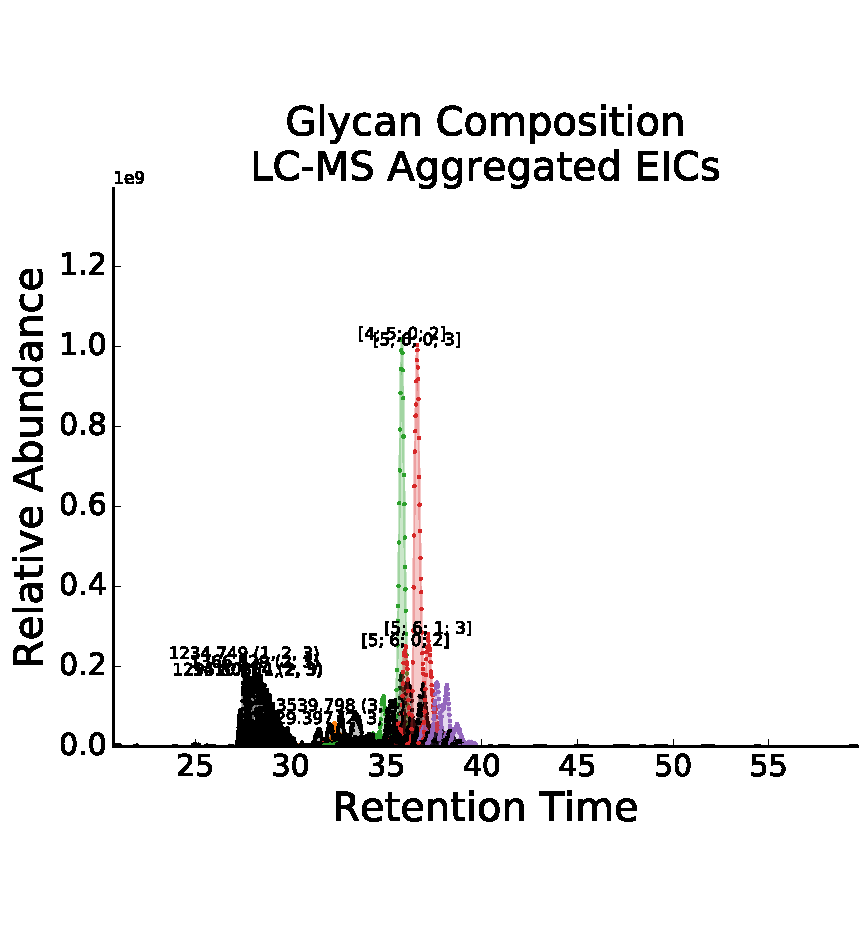
\includegraphics[width=0.45\textwidth,valign=t]{figure/rp_agp_chromatograms.pdf}
        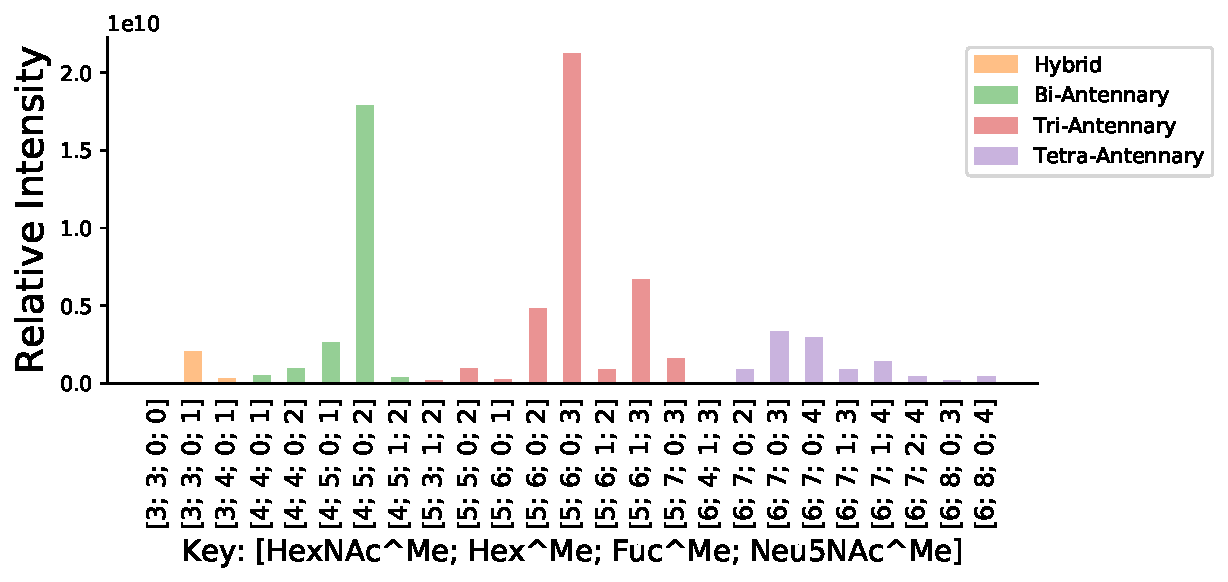
\includegraphics[width=0.45\textwidth,valign=t]{figure/rp_agp_abundances.pdf}
        \caption{\textit{AGP-permethylated-2ul-inj-55-SLens} Glycan Relative Abundances}
        \label{fig:rp_agp_aggregated_eics}
    \end{figure}

    \begin{table}
        \begin{minipage}[t]{0.25\linewidth}
            \vspace{0pt}
            (a)
            \centering
            
    \begin{tabular}{l | c}
        Group & $\tau$ \\
        \hline
        high-mannose & 0.00 \\
        hybrid & 20.22 \\
        bi-antennary & 18.50 \\
        asialo-bi-antennary & 14.15 \\
        tri-antennary & 21.33 \\
        asialo-tri-antennary & 11.71 \\
        tetra-antennary & 16.72 \\
        asialo-tetra-antennary & 1.43 \\
        penta-antennary & 8.13 \\
        asialo-penta-antennary & 0.00 \\
    \end{tabular}
    
            
        \end{minipage}
        \hspace{1cm}
        \begin{minipage}[t]{0.55\linewidth}
            \vspace{0pt}
            (b)
            \centering
            
    \begin{footnotesize}
    \begin{tabular}{l|p{2cm} p{2cm}}
Glycan Compostion &  Unregularized Score &  Regularized Score \\
\hline
\{Hex:3; HexNAc:3\}                   &                13.17 &              16.87 \\
\{Hex:3; HexNAc:3; Neu5NAc:1\}        &                20.04 &              18.03 \\
\{Hex:4; HexNAc:3; Neu5NAc:1\}        &                17.30 &              17.75 \\
\{Fuc:2; Hex:8; HexNAc:3\}            &                 5.85 &               1.01 \\
\{Fuc:1; Hex:9; HexNAc:3\}            &                 1.37 &               0.29 \\
\{Hex:4; HexNAc:4; Neu5NAc:1\}        &                19.72 &              17.30 \\
\{Hex:4; HexNAc:4; Neu5NAc:2\}        &                16.01 &              18.70 \\
\{Fuc:1; Hex:4; HexNAc:4; Neu5NAc:2\} &                 3.49 &               3.49 \\
\{Hex:5; HexNAc:4; Neu5NAc:1\}        &                22.71 &              17.63 \\
\{Hex:5; HexNAc:4; Neu5NAc:2\}        &                24.88 &              19.63 \\
\{Fuc:1; Hex:5; HexNAc:4; Neu5NAc:1\} &                15.95 &              16.71 \\
\{Fuc:1; Hex:5; HexNAc:4; Neu5NAc:2\} &                 7.21 &              17.51 \\
\{Hex:6; HexNAc:4; Neu5NAc:2\}        &                 3.53 &               3.53 \\
\{Fuc:3; Hex:6; HexNAc:4\}            &                 9.22 &              14.52 \\
\{Fuc:2; Hex:7; HexNAc:4; Neu5NAc:2\} &                  nan &              18.98 \\
\{Fuc:1; Hex:8; HexNAc:4; Neu5NAc:2\} &                 5.15 &               0.57 \\
\{Fuc:2; Hex:9; HexNAc:4; Neu5NAc:1\} &                 6.79 &               0.88 \\
\{Fuc:3; Hex:10; HexNAc:4\}           &                 8.29 &               1.65 \\
\{Fuc:1; Hex:3; HexNAc:5; Neu5NAc:2\} &                 7.96 &              16.94 \\
\{Hex:5; HexNAc:5; Neu5NAc:2\}        &                13.88 &              18.23 \\
\{Hex:6; HexNAc:5; Neu5NAc:1\}        &                 8.41 &              12.65 \\
\{Hex:6; HexNAc:5; Neu5NAc:2\}        &                21.65 &              18.71 \\
\{Hex:6; HexNAc:5; Neu5NAc:3\}        &                24.97 &              19.67 \\
\{Fuc:1; Hex:6; HexNAc:5; Neu5NAc:2\} &                11.26 &              17.89 \\
\{Fuc:1; Hex:6; HexNAc:5; Neu5NAc:3\} &                17.38 &              18.64 \\
\{Hex:7; HexNAc:5; Neu5NAc:3\}        &                15.78 &              18.73 \\
\{Hex:7; HexNAc:6; Neu5NAc:2\}        &                10.36 &              15.41 \\
\{Hex:7; HexNAc:6; Neu5NAc:3\}        &                16.80 &              16.03 \\
\{Hex:7; HexNAc:6; Neu5NAc:4\}        &                18.28 &              16.26 \\
\{Fuc:1; Hex:7; HexNAc:6; Neu5NAc:2\} &                 9.17 &              15.42 \\
\{Fuc:1; Hex:7; HexNAc:6; Neu5NAc:3\} &                14.56 &              15.85 \\
\{Fuc:1; Hex:7; HexNAc:6; Neu5NAc:4\} &                19.27 &              16.17 \\
\{Fuc:2; Hex:7; HexNAc:6; Neu5NAc:3\} &                 9.60 &              15.34 \\
\{Fuc:2; Hex:7; HexNAc:6; Neu5NAc:4\} &                10.14 &              15.08 \\
\{Hex:8; HexNAc:6; Neu5NAc:3\}        &                 8.75 &              12.08 \\
\{Hex:8; HexNAc:6; Neu5NAc:4\}        &                 9.87 &              11.96 \\
\{Fuc:1; Hex:8; HexNAc:6; Neu5NAc:4\} &                 5.50 &              11.58 \\
\{Hex:9; HexNAc:7\}                   &                 4.48 &                nan \\
\end{tabular}

    \end{footnotesize}
    
        \end{minipage}
        \caption{
                 Search Results for \textit{AGP-permethylated-2ul-inj-55-SLens}.
                 (a) Estimated $\mathbf{\tau}$ for grid with ${\hat \gamma} = 16.167868$.
                 (b) Scores For Identified Glycans of grid with ${\hat \lambda} = 0.99$.}
        \label{tbl:rp_agp_score_table}
    \end{table}

        \begin{figure}[!htbp]
        \centering
        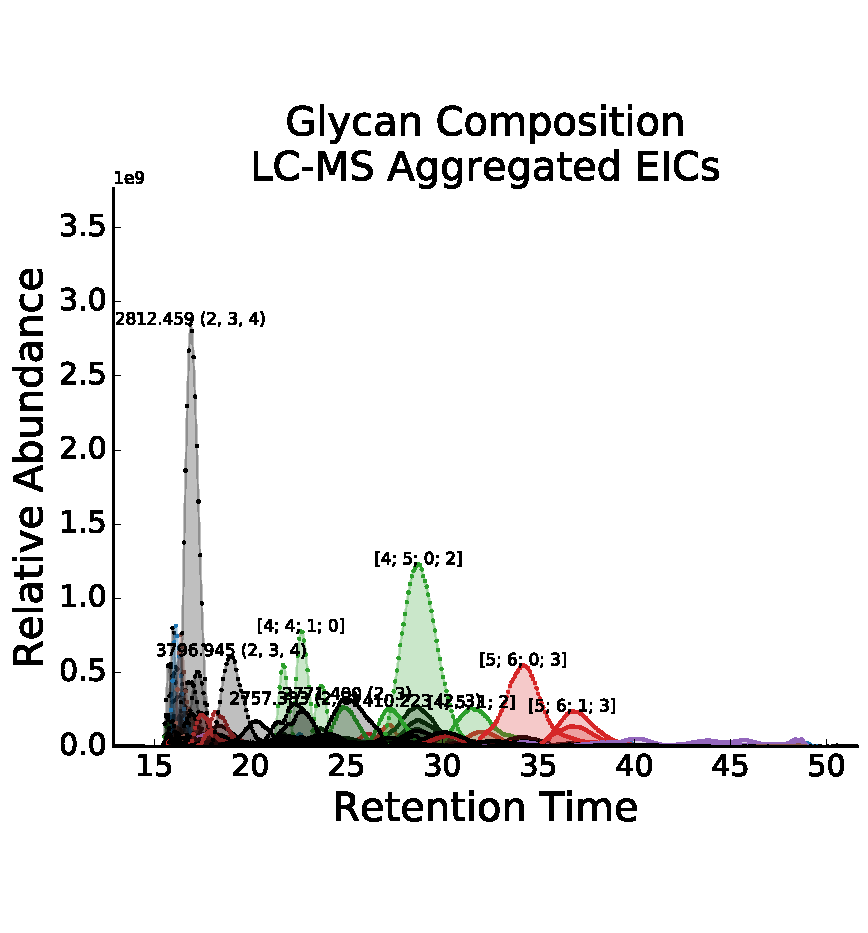
\includegraphics[width=0.45\textwidth,valign=t]{figure/rp_human_serum_chromatograms.pdf}
        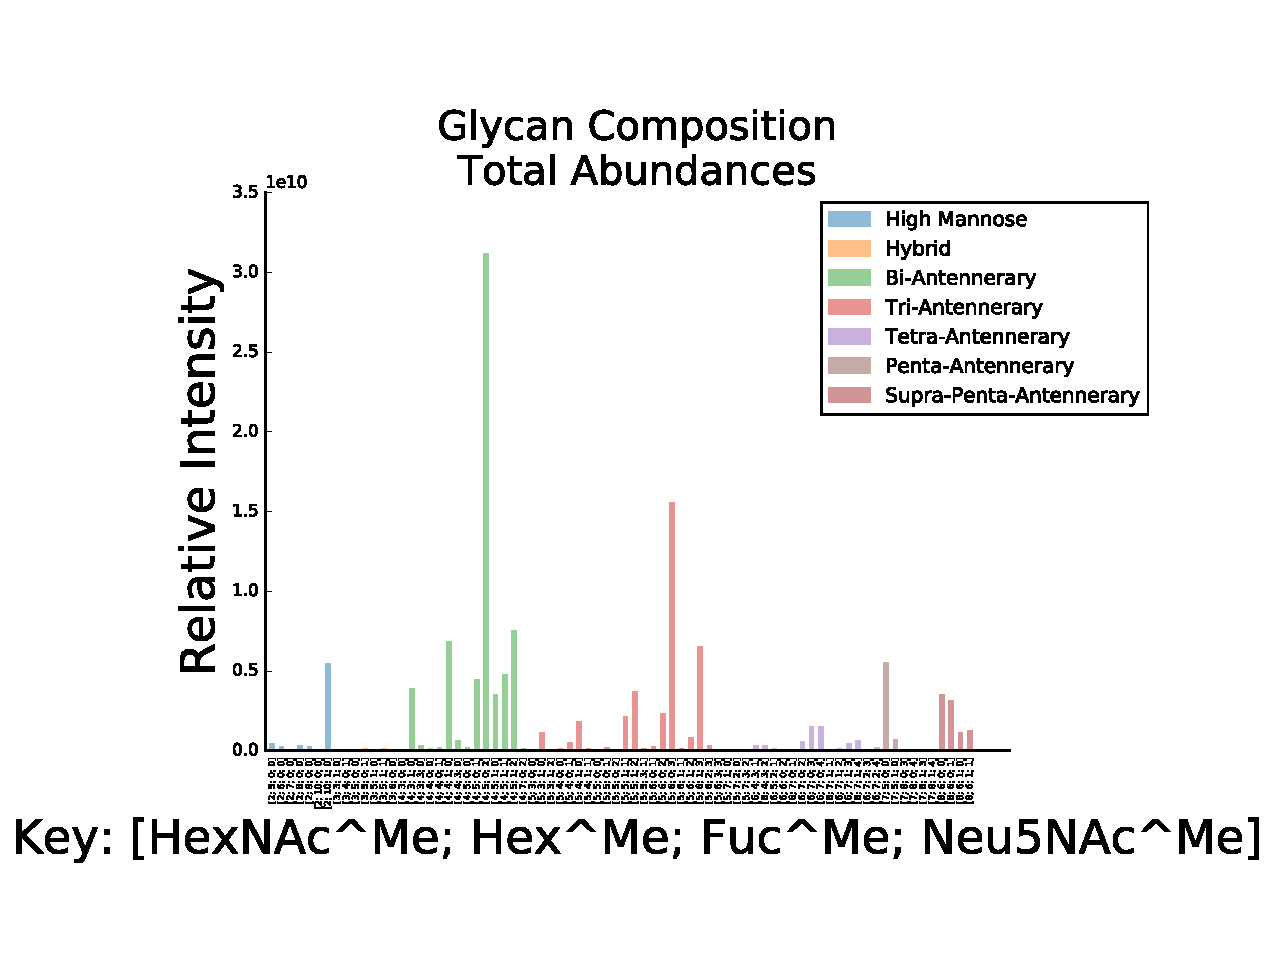
\includegraphics[width=0.45\textwidth,valign=t]{figure/rp_human_serum_abundances.pdf}
        \caption{\textit{Perm-BS-070111-04-Human-Serum} Glycan Relative Abundances}
        \label{fig:rp_human_serum_aggregated_eics}
    \end{figure}

    \begin{table}
        \begin{minipage}[t]{0.25\linewidth}
            \vspace{0pt}
            (a)
            \centering
            
    \begin{tabular}{l | c}
        Group & $\tau$ \\
        \hline
        high-mannose & 20.10 \\
        hybrid & 19.79 \\
        bi-antennary & 18.47 \\
        asialo-bi-antennary & 23.00 \\
        tri-antennary & 22.98 \\
        asialo-tri-antennary & 16.47 \\
        tetra-antennary & 17.52 \\
        asialo-tetra-antennary & 5.92 \\
        penta-antennary & 10.69 \\
        asialo-penta-antennary & 3.56 \\
    \end{tabular}
    
            
        \end{minipage}
        \hspace{1cm}
        \begin{minipage}[t]{0.55\linewidth}
            \vspace{0pt}
            (b)
            \centering
            
    \begin{small}
    \begin{tabular}{l|p{2cm} p{2cm}}
Glycan Compostion &  Unregularized Score &  Regularized Score \\
\hline
\{Hex:5; HexNAc:2\}                   &                22.94 &              20.45 \\
\{Hex:6; HexNAc:2\}                   &                24.33 &              20.77 \\
\{Hex:7; HexNAc:2\}                   &                21.66 &              20.63 \\
\{Hex:8; HexNAc:2\}                   &                21.96 &              20.71 \\
\{Hex:9; HexNAc:2\}                   &                22.02 &              20.31 \\
\{Hex:10; HexNAc:2\}                  &                13.40 &              18.48 \\
\{Fuc:1; Hex:10; HexNAc:2\}           &                15.92 &              18.94 \\
\{Fuc:1; Hex:3; HexNAc:3\}            &                12.75 &              19.71 \\
\{Hex:4; HexNAc:3; Neu5NAc:1\}        &                 6.86 &              17.61 \\
\{Hex:5; HexNAc:3\}                   &                19.17 &              20.27 \\
\{Hex:5; HexNAc:3; Neu5NAc:1\}        &                17.49 &              19.02 \\
\{Fuc:1; Hex:5; HexNAc:3\}            &                13.17 &              19.70 \\
\{Fuc:1; Hex:5; HexNAc:3; Neu5NAc:1\} &                 6.76 &              17.97 \\
\{Hex:6; HexNAc:3\}                   &                13.25 &              19.92 \\
\{Fuc:2; Hex:8; HexNAc:3\}            &                13.62 &               2.60 \\
\{Fuc:2; Hex:10; HexNAc:3\}           &                 8.59 &               2.07 \\
\{Hex:3; HexNAc:4\}                   &                18.15 &              20.31 \\
\{Fuc:1; Hex:3; HexNAc:4\}            &                25.84 &              21.54 \\
\{Fuc:3; Hex:3; HexNAc:4\}            &                16.38 &              20.21 \\
\{Hex:4; HexNAc:4\}                   &                23.30 &              20.00 \\
\{Hex:4; HexNAc:4; Neu5NAc:1\}        &                14.16 &              18.76 \\
\{Fuc:1; Hex:4; HexNAc:4\}            &                25.87 &              20.72 \\
\{Fuc:3; Hex:4; HexNAc:4\}            &                18.07 &              19.41 \\
\{Hex:5; HexNAc:4\}                   &                17.49 &              19.50 \\
\{Hex:5; HexNAc:4; Neu5NAc:1\}        &                22.56 &              19.81 \\
\{Hex:5; HexNAc:4; Neu5NAc:2\}        &                22.25 &              19.77 \\
\{Fuc:1; Hex:5; HexNAc:4\}            &                24.08 &              20.34 \\
\{Fuc:1; Hex:5; HexNAc:4; Neu5NAc:1\} &                22.73 &              19.91 \\
\{Fuc:1; Hex:5; HexNAc:4; Neu5NAc:2\} &                19.52 &              19.67 \\
\{Hex:7; HexNAc:4; Neu5NAc:2\}        &                  nan &              19.71 \\
\{Fuc:2; Hex:9; HexNAc:4; Neu5NAc:1\} &                11.11 &               1.70 \\
\{Fuc:3; Hex:9; HexNAc:4; Neu5NAc:1\} &                 7.84 &               1.65 \\
\{Fuc:3; Hex:10; HexNAc:4\}           &                18.74 &               4.01 \\
\{Hex:3; HexNAc:5\}                   &                12.52 &              20.91 \\
\{Fuc:1; Hex:3; HexNAc:5\}            &                24.17 &              22.85 \\
\{Fuc:1; Hex:3; HexNAc:5; Neu5NAc:2\} &                 6.88 &              16.70 \\
\{Hex:4; HexNAc:5\}                   &                12.73 &              18.75 \\
\{Hex:4; HexNAc:5; Neu5NAc:1\}        &                20.78 &              19.50 \\
\{Fuc:1; Hex:4; HexNAc:5\}            &                23.25 &              20.26 \\
\{Fuc:1; Hex:4; HexNAc:5; Neu5NAc:1\} &                10.53 &              18.77 \\
\{Hex:5; HexNAc:5\}                   &                16.81 &              16.03 \\
\{Hex:5; HexNAc:5; Neu5NAc:1\}        &                16.35 &              17.07 \\
\{Hex:5; HexNAc:5; Neu5NAc:2\}        &                 6.86 &              17.80 \\
\{Fuc:1; Hex:5; HexNAc:5; Neu5NAc:1\} &                21.02 &              17.63 \\
\{Fuc:1; Hex:5; HexNAc:5; Neu5NAc:2\} &                21.99 &              19.43 \\
\{Fuc:3; Hex:5; HexNAc:5; Neu5NAc:1\} &                 6.82 &              15.97 \\
\{Hex:6; HexNAc:5; Neu5NAc:1\}        &                14.77 &              16.50 \\
\{Hex:6; HexNAc:5; Neu5NAc:2\}        &                18.97 &              18.82 \\
\{Hex:6; HexNAc:5; Neu5NAc:3\}        &                23.46 &              20.04 \\
\{Fuc:1; Hex:6; HexNAc:5; Neu5NAc:1\} &                10.92 &              16.06 \\
\{Fuc:1; Hex:6; HexNAc:5; Neu5NAc:2\} &                11.56 &              18.34 \\
\{Fuc:1; Hex:6; HexNAc:5; Neu5NAc:3\} &                24.83 &              19.92 \\
\{Fuc:2; Hex:6; HexNAc:5; Neu5NAc:3\} &                11.41 &              18.06 \\
\{Fuc:3; Hex:6; HexNAc:5; Neu5NAc:3\} &                 8.65 &              17.66 \\
\{Fuc:1; Hex:7; HexNAc:5\}            &                 5.29 &              10.24 \\
\{Fuc:2; Hex:7; HexNAc:5\}            &                 6.54 &              10.34 \\
\{Fuc:3; Hex:3; HexNAc:6\}            &                 6.57 &               0.83 \\
\{Fuc:3; Hex:4; HexNAc:6; Neu5NAc:1\} &                 9.45 &              17.52 \\
\{Fuc:3; Hex:4; HexNAc:6; Neu5NAc:2\} &                 4.93 &              20.56 \\
\{Fuc:2; Hex:5; HexNAc:6; Neu5NAc:1\} &                 7.87 &              13.83 \\
\{Hex:6; HexNAc:6; Neu5NAc:2\}        &                 7.92 &              16.62 \\
\{Fuc:1; Hex:6; HexNAc:6; Neu5NAc:4\} &                 1.95 &               1.95 \\
\{Hex:7; HexNAc:6; Neu5NAc:1\}        &                 4.73 &              10.47 \\
\{Hex:7; HexNAc:6; Neu5NAc:2\}        &                12.75 &              16.69 \\
\{Hex:7; HexNAc:6; Neu5NAc:3\}        &                16.51 &              17.53 \\
\{Hex:7; HexNAc:6; Neu5NAc:4\}        &                27.88 &              19.15 \\
\{Fuc:1; Hex:7; HexNAc:6; Neu5NAc:1\} &                 4.62 &              10.46 \\
\{Fuc:1; Hex:7; HexNAc:6; Neu5NAc:2\} &                10.71 &              16.62 \\
\{Fuc:1; Hex:7; HexNAc:6; Neu5NAc:3\} &                15.40 &              17.10 \\
\{Fuc:1; Hex:7; HexNAc:6; Neu5NAc:4\} &                18.08 &              17.45 \\
\{Fuc:2; Hex:7; HexNAc:6; Neu5NAc:3\} &                 8.07 &              16.43 \\
\{Fuc:2; Hex:7; HexNAc:6; Neu5NAc:4\} &                19.85 &              17.63 \\
\{Hex:5; HexNAc:7\}                   &                16.12 &               8.09 \\
\{Fuc:1; Hex:5; HexNAc:7\}            &                13.72 &               7.44 \\
\{Hex:8; HexNAc:7; Neu5NAc:3\}        &                10.83 &              13.57 \\
\{Hex:8; HexNAc:7; Neu5NAc:4\}        &                16.66 &              14.28 \\
\{Fuc:1; Hex:8; HexNAc:7; Neu5NAc:3\} &                 7.55 &              13.09 \\
\{Fuc:1; Hex:8; HexNAc:7; Neu5NAc:4\} &                 8.84 &              13.33 \\
\{Fuc:1; Hex:9; HexNAc:7\}            &                 4.69 &               3.76 \\
\{Hex:5; HexNAc:8\}                   &                12.94 &               2.90 \\
\{Fuc:1; Hex:5; HexNAc:8\}            &                 5.06 &               1.52 \\
\{Hex:6; HexNAc:8\}                   &                16.72 &               6.73 \\
\{Hex:6; HexNAc:8; Neu5NAc:1\}        &                15.58 &               7.83 \\
\{Fuc:1; Hex:6; HexNAc:8\}            &                10.57 &               5.49 \\
\{Fuc:1; Hex:6; HexNAc:8; Neu5NAc:1\} &                15.36 &               7.42 \\
\{Hex:6; HexNAc:9\}                   &                 6.16 &               2.25 \\
\{Hex:7; HexNAc:9\}                   &                10.12 &               2.64 \\
\{Hex:7; HexNAc:9; Neu5NAc:1\}        &                 7.97 &               2.38 \\
\{Hex:7; HexNAc:9; Neu5NAc:2\}        &                14.36 &               2.91 \\
\{Fuc:1; Hex:7; HexNAc:9; Neu5NAc:1\} &                 6.50 &               1.91 \\
\{Fuc:1; Hex:7; HexNAc:9; Neu5NAc:2\} &                16.90 &               2.87 \\
\end{tabular}

    \end{small}
    
        \end{minipage}
        \caption{
                 Search Results for \textit{Perm-BS-070111-04-Human-Serum}.
                 (a) Estimated $\mathbf{\tau}$ for grid with ${\hat \gamma} = 18.199966$.
                 (b) Scores For Identified Glycans of grid with ${\hat \lambda} = 0.935$.}
        \label{tbl:rp_human_serum_score_table}
    \end{table}



% \section{Discussion}

    We demonstrated that the regularization method improved the
    sensitivity and specificity of glycan composition assignment for
    LC-MS based experiments. The method used similar assumptions about
    the importance of common substructural elements of \nglycans to
    \cite{Goldberg2009}, but we extend this concept with the addition
    of a procedure for learning the relationship strengths and use
    broader groups of structures.

    The experimental results from the original analysis of \philbs and
    \phil82 demonstrated that while both strains expressed predominantly
    high-mannose glycosylation, \philbs expressed more larger complex-type
    structures (\cite{Khatri2016a}). In our findings shown in Figure~\ref{fig:philbs_assignments},
    we recapitulate these results while reducing the number of false
    assignments, Table~\ref{tab:philbs_statistics}. There are substantial
    differences in both the mass spectral processing and scoring schemes which
    contribute to these results, but the regularization procedure is responsible
    for recovering many low abundance features from this comparison. As these
    samples are derived from chicken eggs, we have observed larger
    branching patterns than are observed in normal mammalian tissue (\cite{Stanley2009}).
    There is evidence for this in the \philbs with \textbf{HexNAc9 Hex10}-based compositions
    suggesting a seven branch pattern, though this cannot be determined without high quality
    \msn data. The $\mathbf{\tau}$ fit for Phil-BS (shown) and Phil-82 (supplement) have
    smaller values in the neighborhoods of their largest glycan compositions as
    these features tended to be low in abundance and not high scoring in their own
    right, but were partially supported by the overlap with the next largest neighborhood,
    as expected. We observed the best performance with the \textit{Combinatorial + Sulfate}
    database, which produced more than half-again as many true matches than the other two
    databases. It produced several false matches as well, but the smoothing process removed
    these while boosting the score of other low abundance matches which were consistent with
    higher scoring matches.

    The Krambeck database performed identically in all smoothing conditions as it
    was only able to match the common species, not including cases that were multiply
    fucosylated or sulfated. It had no false matches ranked alongside its true matches so
    smoothing could not change its performance. The \glyspace-derived database produced more true
    matches, but also lacked some of these more fucosylated and complex compositions. Some of the
    compositions included by the \glyspace-derived database were lower scoring, but the chosen
    value of $\gamma$ for that database was greater than 18, causing the fitted values of $\mathbf{\tau}$
    omit the larger, less abundant complex-type \nglycans. This caused smoothing to lower the scores
    of these real matches rather than raise them, as with the \textit{Combinatorial + Sulfate} database.

    As we show in Figure~\ref{fig:rpserum_perf}, regularization improves the
    predictive performance of the identification algorithm on \rpserum for all databases.
    We reproduce the majority of the glycan assignments from \cite{Yu2013}, but the ambiguity
    caused by ammonium adduction as shown in Figure~\ref{fig:rpserum_assignment:c} makes a
    direct comparison of composition assignment lists difficult. Our algorithm requires a minimum
    amount of MS1 information in order to compute a score, which some of the assignments in the
    original published results do not possess, which are omitted from the count in Table~
    \ref{tab:serum_statistics}. After accounting for ambiguity, we were able to assign all
    of the compositions previously reported using the Krambeck database, which was used
    by \cite{Yu2013}, and with the combinatorial database. The \glyspace-derived database did not
    contain all of these compositions, but performed competitively with the combinatorial
    database's ROC AUC. The combinatorial database contained a small number of glycan compositions
    which were not in Krambeck but which were consistent with other glycan compositions
    observed nearby in retention time. The combinatorial database also benefited most
    substantially from smoothing, discarding many false positives while retaining many more
    true positives at the same false positive rate compared to the other databases. These
    invalid glycan compositions can match LC-MS features at any point in the elution profile,
    though in this dataset the majority of these matches appear to be in the time range between
    10 and 22 minutes, and similar glycan compositions that are biosynthetically valid elute
    later on in the experiment. Therefore a for a retention-time aware approach to evaluating glycan
    composition assignments, as described in \cite{Hu2016} could also be useful, but this is
    likely dependent upon the experimental workup and separation technique used.

    While the biosynthetically constrained Krambeck database performed better on \rpserum,
    it did not contain all of the reasonably assignable glycan compositions, and it performed
    poorly on \philbs with a false negative rate of 50\% compared to the combinatorial database.
    This is because the necessary enzymatic pathways were either not considered in the original
    authors' model because either the enzyme was excluded for simplicity (\cite{Krambeck2009}) or
    because the particular enzymes used were not within the scope of the model used
    (\cite{Spiro2000,Ichimiya2014}). This highlights the importance of selecting a good reference
    database, though a post-processing step such as the we described here can help mitigate using
    too large a database, but not a too small one.

    In this work, we used the same network neighborhood imposed over different underlying sets of
    composition nodes, and the connectivity of those networks did not take into account the biosynthetic
    process. It may be possible to obtain better performance by defining network connectivity according
    to enzymatic relationships. This may also alter how the neighborhoods are defined and how $\mathbf{A}$
    is parameterized, and in turn how $\mathbf{\tau}$ is learned. Similarly, this procedure depends upon
    the scoring functions used, so selecting another set of functions for the data to fit may lead
    to different parameter values.

    Lastly, while these case studies have demonstrated the algorithm's ability to learn network parameters
    from the data, an expert can define $\mathbf{\tau}$ and $\mathbf{A}$ themselves or obtain a model fitted
    on related data and apply it directly without a fitting step. An expert could use this model specification
    to impose prior beliefs on the evaluation process, and adjust $\lambda$ to control the importance of
    the these beliefs. Similarly, one could also use the derivation of ${\hat \phi_m}$ to estimate the score
    for an unobserved glycan composition, given $\mathbf{A}$ and $\mathbf{\tau}$.

    We used our glycoinformatics toolkit to produce a richer abstraction of glycans and monosaccharides,
    including producing standard-compliant textual representations of these structures and compositions.
    We produced a text file containing all of the glycan compositions found in the Krambeck and Combinatorial
    database but not the \glyspace-derived database in the above samples (see supplemental information
    \ref{S-sec:glyspace_integration_and_upload}),
    and have submit it to GlyTouCan (\cite{Tiemeyer2017}) for registration so that future researchers can
    use these structures.

\section{Conclusions}
    In this study, we demonstrated the advantages of our application of Laplacian
    Regularization to smooth LC-MS assignments of glycan compositions across multiple
    experimental protocols (\cite{Hu2012, Khatri2016a}). Our algorithm's performance is
    competitive with existing tools for analyzing the same type of data, with the added
    benefit of more flexible evaluation process and broader range of understood monosaccharides.
    Our tools integrate with \glyspace and allows users to leverage existing glycomics
    repositories to build databases where applicable.

    All of the methods demonstrated in this paper are available as part of the open source,
    cross-platform glycomics and glycoproteomics software \texttt{GlycReSoft}, freely
    available at \href{http://www.bumc.bu.edu/msr/glycresoft/}{http://www.bumc.bu.edu/msr/glycresoft/}.



\bibliographystyle{natbib}
\bibliography{bibliography}

\end{document}